\chapter{Introduction\label{chap:intro}}

\begin{remark}{Outline}
In this chapter, we introduce fundamental concepts of molecular evolution and describe how they are integrated into the field of phylodynamics, a discipline that describes the interaction of evolutionary and ecological dynamics underlying pathogen spread.
Different viral pathogens that have emerged in recent history illustrate the vulnerability of the human population to pandemic threats.
We stress the importance of developing efficient and statistically sound surveillance methods that can assist in characterizing those threats.

We subsequently describe some of the most important breakthroughs in the history of methods and models to study molecular evolution, such as the introduction of a molecular clock which allows dating divergence events from genetic data and historical calibration points or sampling times, the shift of the field towards probabilistic methods, the advent of Monte Carlo algorithms as well as powerful and increasingly more attainable computer hardware, which have facilitated the adoption of Bayesian approaches.
We further explain how these advances - implemented into publicly available software - adequately account for phylogenetic uncertainty by averaging over all plausible evolutionary histories.

Finally Subsection~\ref{sub:objectives} positions the work presented in this thesis and outlines how it advances our understanding of the processes shaping viral evolution and spread.
The additional sections of this introductory chapter are devoted towards describing the basic inference methodology in more detail, and constitute the background knowledge for the work presented in Chapters~\ref{chap:epoch}--\ref{chap:pibuss}.
\end{remark}

\section{General Introduction\label{sub:general}}

\subsection{Viral epidemiology and the emergence of phylodynamics\label{sub:epidemiology}}

Many pathogens represent a clear and eminent threat to public health. 
This has been exemplified by the outbreak of the Severe Acute Respiratory Syndrome (SARS) in China \citep{Ksiazek2003}, the H1N1 swine-origin influenza A virus outbreak in 2009 \citep{Fraser2009}, which attained pandemic status in only a few months time, but also more recently by a large outbreak of the Ebola haemorrhagic fever in humans in West Africa \citep{Dudas2014}. 

Many studies on emerging infectious diseases (EIDs) have highlighted viral pathogens as a major threat to the public health, owing to their high rates of nucleotide substitution, and therefore high capacity to adapt to new hosts. 
Due to highly intensified human mobility there are virtually no natural barriers for the spread of human RNA viruses \citep{Brockmann2006}.
In recent decades, EIDs are becoming increasingly widespread, with their impact and spread only rising over time \citep{Jones2008}.
This may not be surprising since it is well-acknowledged that disease emergence is largely a product of anthropogenic and demographic changes, making it a hidden cost of human economic development.
 
Combating viral spread and its associated disease burden is a tremendous challenge requiring significant research efforts and decided public health measures. 
Viral sequence data has been recognized as a major asset in the characterization of pathogens that threaten public health.
Molecular epidemiology complements traditional epidemiological studies because it primarily focuses on the etiological agent rather than the host \citep{Leitner2002}.
In particular, the historical information contained in viral gene sequences contributes to a better insight in emergence and early transmission dynamics, even before systematic epidemiological surveillance has been initiated. 
For many years, phylogenetic analysis has been the primary tool in molecular epidemiology. 
By reconstructing a phylogenetic tree, we are able to study the evolutionary history of viral strains, assess epidemiological linkage amongst them, and shed light on transmission patterns. 
With the advent of high-throughput DNA sequencing, genomic data from RNA viruses is becoming available in unprecedented quantities and with remarkable rapidity. 

The last decade has witnessed a particular focus of analyses of viral evolutionary dynamics on integrating concepts of phylogenetic and epidemiological dynamics, a research direction originally coined `phylodynamics' \citep{Grenfell2004}.
By aiming at the development of a full quantitative understanding of the processes that shape the epidemiology and evolution of RNA viruses, phylodynamics has become a burgeoning area of research \citep{Holmes2009}.
In order to perform comprehensive and quantitative analyses of the interaction between the ecological and evolutionary dynamics of RNA viruses, new computational developments are needed and some of these are actively bridging the gap with the field of mathematical epidemiology.

Advances in epidemiological modeling have made it possible to describe the transmission of contagions through individuals.
Perhaps the simplest and best-studied model is the ${\mathcal{S} \rightarrow \mathcal{I} \rightarrow \mathcal{R}}$  compartmental model % TODO: citation
, which describes how (S)usceptible individuals become (I)nfected and the (R)ecover, as a function of time.  
These models can be extended to include birth and death events % TODO: citation
and are instrumental in finding the number of secondary infections caused by a single infected individual in an entirely susceptible population, a basic reproductive quantity denoted by $R_{0}$.
This quantity determines whether an epidemic is occurring or whether the spread of the disease will die out.
Traditionally, parameters in these models were inferred using surveillance data, %yet more complicated epidemiological studies involving e.g. seasonality, multiple populations with varying $R_0$ or other possible epidemiological predictors are often analytically intractable.
%In that light, developments to infer parameters of compartmental models by studying 
but increasingly pathogen genetic data is being used to inform SIR model parameters \citep{Volz2009}.
%molecular sequence data have become increasingly important \citep{Volz2009}.
Further, patterns of geographic diffusion of infectious diseases can be inferred from sequence data \citep{Lemey2009}, sometimes in combination with information on the host movement \citep{Lemey2014}. 
Integrating population structure into compartmental models which explicitly track the transmission between the infected individuals can provide new avenues for inferring patterns of viral spread \citep{Rasmussen2014}.

Whereas for emerging pathogens modeling efforts are typically focused on providing estimates of the basic reproduction number, for ongoing epidemics one is typically interested in quantifying the effects of control and preventive measures on between-host scales and the effect of treatment on a within-host scale.
In that respect it is important to characterize adaptive evolution, 
%For that reason most efforts are focused on reliable detection of adaptive selection pressure,
a major driving force of viral evolution.
\cite{Volz2013} report nine Influenza A H1N1 vaccine updates being recommended by the World Health Organization (WHO) between 1978 and 2009, as compared to 20 updates recommended for Influenza H3N2, suggesting that the latter undergoes much more adaptive evolution that the former.
Unfortunately positive selection is notoriously difficult to detect, as on the sequence level it may apply to only a handful of sites, on the tree topology level it may apply to only some of the branches, or even only to a particular time on that branch.
A substantial amount of work has been aimed at developing models which can detect selection acting differently between sites, between branches or between a combination of those \citep{NY98, Pond2005a, Goode2008}.

In order to position the work presented here, we first provide a brief general account of the field of molecular evolution and phylogenetics and then introduce recent developments and models proposed specifically for rapidly-evolving RNA viruses, and how this has culminated in to a state-of-the-art statistical framework for phylodynamics.
As a final part of the general introduction, we outline how the current doctoral thesis work extends and complements this framework in the objectives.
The remainder of the chapter provides a more mathematically-oriented description of how to model evolution as a stochastic process on trees, the computational aspects involved, and how to treat the problem from a Bayesian statistical perspective.

\subsection{Molecular evolution and phylogenetics\label{sub:molevol}}

Evolution is the product of mutational processes that stochastically introduce changes into the genetic make-up of organisms and population processes that lead to the elimination, fixation or partial maintenance of these mutations in the population.
The latter occurs through genetic drift or the more deterministic process of natural selection. 
Adaptation by natural selection is the most important process in biology as it determines the fate of mutations that impact the fitness of the organisms within their variable environment.
 
Molecular phylogenetics studies the evolutionary pathways underlying these processes that lead to the polymorphism data observed in contemporary times.
Based on the sequence data obtained for a number of organisms or taxa, molecular phylogenetics aims at inferring the ancestral relationships and evolutionary parameters of interest.
The result of a molecular phylogenetic analysis is represented in a phylogenetic tree. 
Phylogenetic trees are bifurcating graphs depicting the pattern of common ancestry among the taxa.
External nodes, tips or leafs in the tree represent the observed character data, while internal nodes represent the missing data for hypothetical ancestors.  
The common ancestor of all the observed character sequences (the most-recent common ancestor, MRCA) is referred to the as the root of the tree.
In unrooted trees, the position of the root is unknown, and unlike rooted trees, they are therefore lacking an evolutionary direction.
A group of taxa in a phylogeny, consisting of all the descendants sharing a particular ancestor, is called a clade or phylogenetic cluster.

%---FIRST TREES---%
\begin{figure}[h!]
\centering
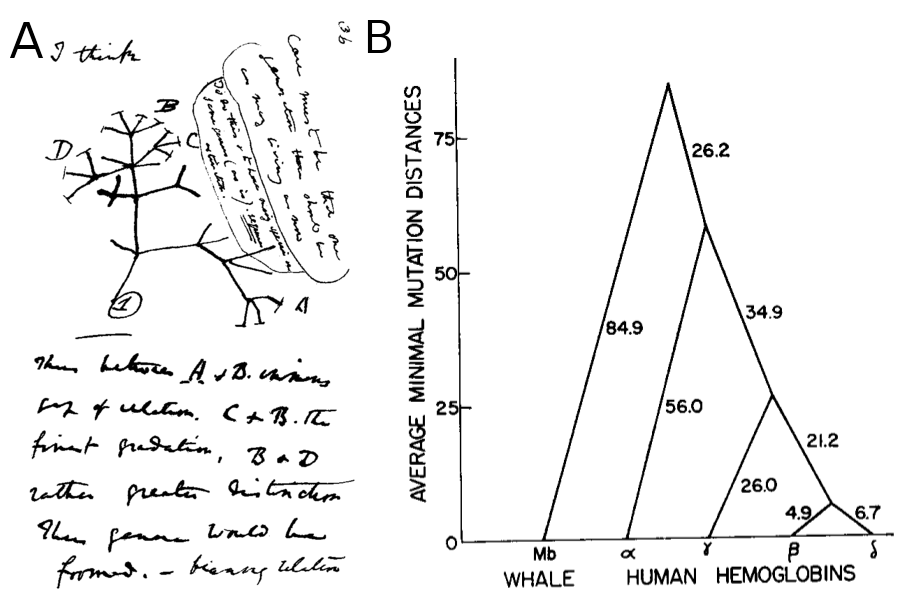
\includegraphics[scale=0.6]{first_trees} 
\caption{
{ \footnotesize 
{\bf Phylogenetic trees.} A. A page from Darwin's notebooks around July 1837 showing his first sketch of an evolutionary tree.
B. First phylogeny estimated from genetic data and published by \cite{Fitch1967}.
}% END: footnotesize
}
\label{fig:first_trees}
\end{figure}

%Underlying assumption of the phylogenetic tree is that the data used to infer them indeed encompasses some sort of evolutionary relatedness.
Phylogenetic thinking traces back to the first known figure of a phylogenetic tree, sketched by Charles Darwin in 1837 on the margin side of his notebook (see Figure \ref{fig:first_trees}), with the famous words \emph{`I think'} written above it.
In those days there was no notion of genetic data, therefore Darwin conceived his trees by comparing morphology, assuming that organisms with similar forms and shapes descended from more recent common ancestors. %\footnote{Furry with furry.}.
Modern phylogenetics use molecular data and a combination of statistical and computational methods to reconstruct phylogenetic trees.
%distance-based trees
Among the first tractable methods to reconstruct trees from molecular data were the hierarchical clustering methods based on genetic distance \citep{Fitch1967}, defined as the number of nucleotides that would need to be altered to make two sequences identical (see Figure \ref{fig:first_trees} B).
These methods were criticized for not making explicit use of the relationship between individual characters of the genetic data, but rather reducing it to distance-based measures.
%Moreover by using pairwise comparisons some of the information is inevitably lost.
Moreover, hierarchical clustering leads to a single point estimate of the evolutionary history and therefore does not consider alternative hypotheses for the data.

% parsimony
In order to evaluate different tree topologies the idea of parsimony was adopted in phylogenetics. 
Maximum parsimony approaches attempt to find the tree that requires the minimum number of evolutionary changes to explain the data. %, maing use of the whole data at once.
This concept stems from the work of William of Ockham (1320), who stated that among competing hypotheses one should select the simplest one and disregard the remaining more complex ones (Ockham's razor).
\cite{Edwards1963} formally introduced the idea into phylogenetics.
Later, \cite{Fitch1971} published an dynamic programming algorithm that efficiently searches all possible tree topologies, assigning scores to them and finding the one with minimal parsimony score.
Figure \ref{fig:parsimony} presents an example of parsimony, where among two trees explaining the evolution of sequences {\color{green}AAG}, {\color{green}AAA}, {\color{green}GGA}, {\color{green}AGA} only the most parsimonious one is selected.

%---PARSIMONY TREE---%
\begin{figure}[h!]
\centering
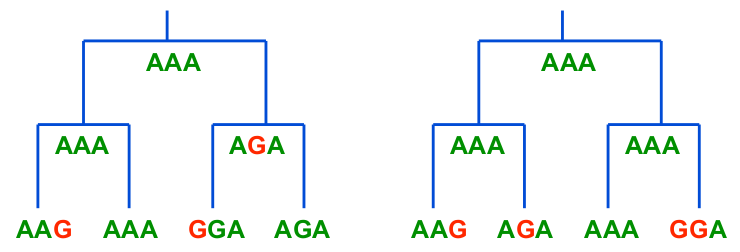
\includegraphics[scale=0.3]{parsimony} 
\caption{
{ \footnotesize 
{\bf Parsimony example.} The tree on the left is preferred as it requires the least amount of changes (3 substitutions as opposed to 4 for the tree on the right).
}% END: footnotesize
}
\label{fig:parsimony}
\end{figure}

%likelihood
As a statistical alternative to an optimality criterion, the likelihood had also been proposed for phylogenetic inference relatively early.
The idea of using maximum likelihood to estimate evolutionary trees was first proposed by \cite{Edwards1964}, although without a working implementation at the time of the publication.
Maximum likelihood is a probabilistic method of inference, that evaluates a hypothesis in terms of how probable it is in the light of the observed data.
In a phylogenetic setting, the likelihood function returns the probability that the proposed model and the proposed tree, understood as a topology and branch lengths, have generated the observed data.
\myedit{svthree}{
In general an evolutionary history and associated set of evolutionary parameters with higher probability of generating the observed data is naturally preferred over a history with a lower probability of generating it.
By using optimization techniques one can find the parameter values that maximize the probability of observing the data.
}
% The evolutionary history and associated set of evolutionary parameters with a higher probability is naturally preferred over a history with a lower probability.
% By using optimization techniques one can find the parameter values that maximize the probability of observing the data.
In his influential work, \cite{Felsenstein1981} proposed an efficient algorithm for calculating a likelihood of sequence evolution on a tree under an evolutionary model of substitution, the so called `tree pruning' algorithm.
Unfortunately finding the maximum likelihood tree requires a search through the space of all possible tree topologies; in section \ref{sub:mlburden} we discuss in detail the computational burden associated with these calculations.
The effort required to exhaustively search through a space of all possible rooted trees grows explosively with the number of taxa, as depicted in Table \ref{tab:maxLikeBurden}.

\begin{table}[h!]
\centering
% \footnotesize{
\begin{tabular}{cc}
% {@{}l*{2}{D{.}{.}{7}}@{}}
\hline 
Tips & Rooted trees $\frac{(2N-3)!}{2^{N-2}\cdot(N-2)!}$ \tabularnewline
\hline 
\rowcolor{gray1}
$3$ & $3$\tabularnewline
$6$ & $945$\tabularnewline
\rowcolor{gray1}
$9$ & $2'027'025$\tabularnewline
$15$ & $2\times10^{14}$\tabularnewline
\rowcolor{gray1}
$20$ & $8\times10^{21}$\tabularnewline
$55$ & $3.19\times10^{86}$\tabularnewline
\end{tabular}
% }
\caption{
{ \footnotesize 
{\bf{Number of rooted trees per number of taxa.}} For comparison, $4 \times 10^{80} $ is the number of atoms in the observable universe.
}% END: footnotesize
}
\label{tab:maxLikeBurden}
\end{table}

%bayesian
The advent of powerful and increasingly more attainable computing power has been instrumental to the adoption of statistical methods based on likelihood estimation and the closely related Bayesian methods.
Bayesian statistical thinking is not a new idea and stems back to the XVII century works of reverend Thomas Bayes, a statistician, philosopher and theologian. 

\clearpage

%---BAYES---%
\begin{remark}{Thomas Bayes}
\begin{figure}[H]
\centering
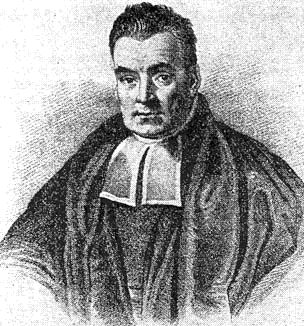
\includegraphics[scale=0.4]{Thomas_Bayes} 
\caption{
{ \footnotesize 
{\bf Only known portrait of reverend Thomas Bayes.} This portrait was published in the 1936 book on the history of actuarial science `History of Life Insurance'. It is only hypothesised to be an actual portrait of the scholar.
}% END: footnotesize
}
\label{fig:bayes}
\end{figure}
\end{remark}

Interestingly, Bayes has never published his famous work.
Bayesian statistics has always been appealing as a very flexible approach to inference, as it allows for inclusion of prior belief about any unknown parameters, which, combined with the likelihood of the data, forms an `updated' view of the model, the so-called posterior distribution.
This prior specification can reflect the degree of uncertainty we put into our belief and can be further enhanced by the use of the so called hyperpriors, prior distributions put on the parameters of first order priors.
Moreover, Bayesian inference allows for a natural interpretation of the results in terms of probability distributions. 
Unfortunately, calculating a posterior distribution requires the computation of integrals over the space of all possible parameter values, which are often multi-dimensional.
For a long time, this has limited its use for most but the simplest problems until \cite{Metropolis1953} proposed a Markov chain Monte Carlo (MCMC) algorithm for obtaining a sequence of random samples from a probability distribution for which direct sampling is difficult. 
Later, \cite{Hasting1970} extended and generalized the algorithm which came to be known as the Metropolis-Hastings method.

\begin{remark}{Monte Carlo}
Monte Carlo methods are computational algorithms that rely on computer-generated pseudo-random numbers to obtain numerical results. 
They were invented in the late 1940's by Stanis\l{}aw Ulam, while he was working on nuclear weapons for `project Manhattan'
at the Los Alamos laboratory.  
It was named after the Monte Carlo Casino in Monaco, where Ulam's uncle often gambled.
Monte Carlo was dubbed the most important algorithm of 21st century by the Society for Industrial and Applied Mathematics (SIAM).
\end{remark}

The Bayesian inference problem can be formulated as a sampling problem, as we discuss in Section \ref{sec:bayesian_inference}, reducing to a very simple and effective method, which contributed to the popularity of Bayesian statistics that we see today. 
The availability of programs for Bayesian phylogenetics like MrBayes \citep{Huelsenbeck2001} and BEAST \citep{Drummond2012} further contributed towards the widespread adoption and popularity of these methods in evolutionary biology.

\subsection{Time-calibrated trees and Measurably Evolving Populations\label{sub:clocks}}

%Molecular clock
The molecular clock hypothesis (\cite{Zuckerkandl1962}) posits that the rate of evolution of any specified protein remains roughly constant over time and over different lineages.
In particular, Zuckerkandl and Pauling observed that amino acids were replaced at a roughly constant rate in hemoglobins as judged from the fossil record.

% \begin{figure}[H]
% \centering
% 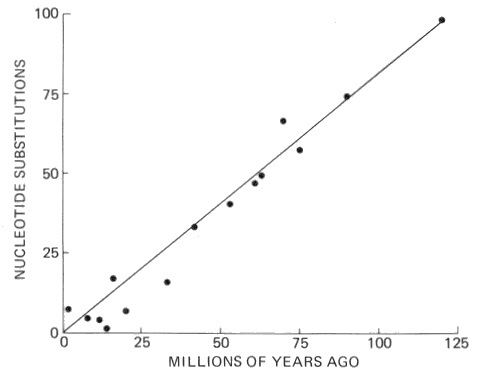
\includegraphics[scale=0.3]{molecular_clock} 
% \caption{
% { \footnotesize 
% {\bf Inferred pairwise nucleotide substitutions among 17 mammal species plotted against dates of divergence estimated from fossil records \citep{Wilson1976}.} Linear relationship suggests that pairwise molecular differences are proportional to the time of their separation, and not the morphological traits.
% }% END: footnotesize
% }
% \label{fig:molecular_clock}
% \end{figure}

This hypothesis is compelling because of its simplicity and because it provides a means to date bifurcation events on the tree of life.
A molecular clock assumption can only result in estimates of the proportion of time between two events. 
To estimate concrete dates for phylogenetic nodes, it needs to be calibrated using historical information such as  fossil records.
% MEPs
For rapidly evolving viruses however, it is possible to sample sequences that diverge over an observable timescale. 
As opposed to the ultrametric topology assumed for slowly evolving organisms (Figure~\ref{fig:ultrametric}), the dates of the samples themselves can be used to calibrate the molecular clock \citep{Rambaut2000}.

%---SAMPLING SCHEMES---%
\begin{figure}[h!]
\centering
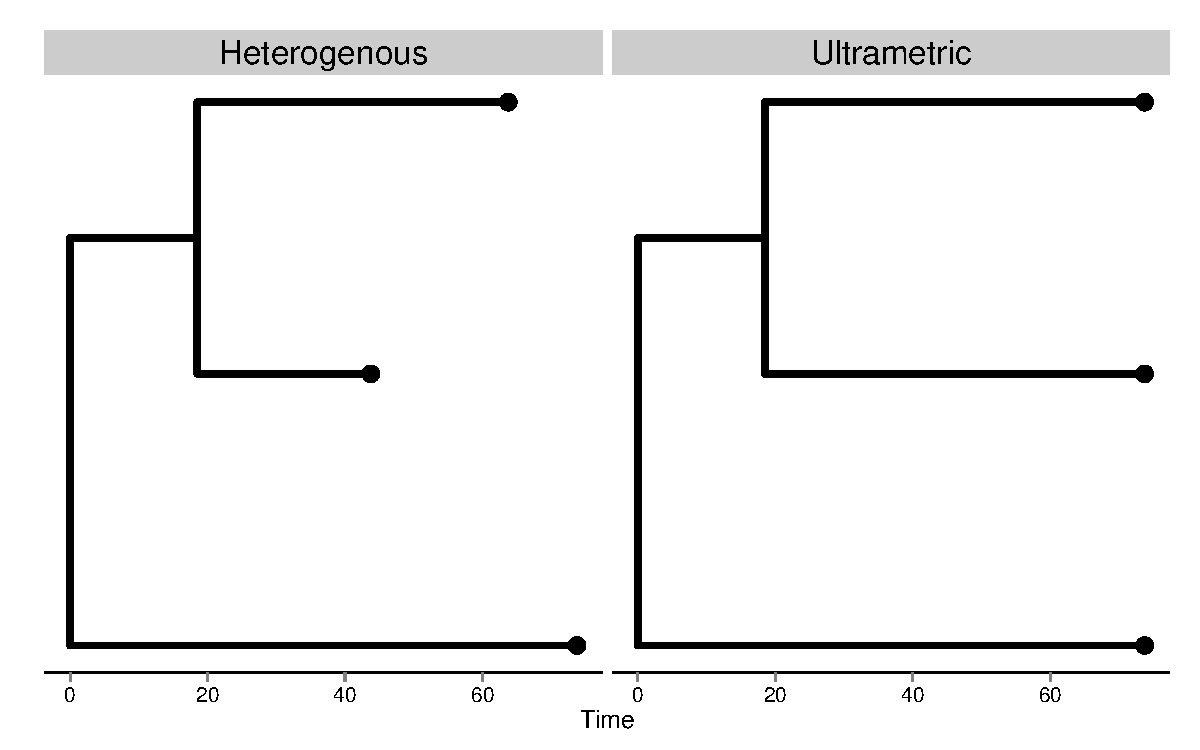
\includegraphics[scale=0.3]{ultrametric} 
\caption{
{ \footnotesize 
{\bf Different tree structures imposed by molecular clock assumptions for organisms evolving at different rates.} 
The tree on the right represents an evolutionary history of slowly evolving organisms, and has tips sampled in the last decades that are all aligned at $t=0$. 
Conversely the tree on the left represents an evolutionary history of rapidly evolving organisms with samples at different points in time in the last decades. 
By enforcing tip heights to be proportional to their sampling dates, temporal information is provided to calibrate the molecular clock for rapidly evolving organisms.
}% END: footnotesize
}
\label{fig:ultrametric}
\end{figure}

Time-stamped data sets have also been referred to as heterochronous data and %frequently arise from studies involving viruses which accumulate large amounts of genetic change in a relatively short amount of time.
populations for which such data can be obtained are called measurably evolving populations (MEPs, \cite{Drummond2003}).
This concept has been instrumental for providing estimates of evolutionary rates and for further developments in molecular clock modelling \citep{Drummond2006}.

% relaxed phylogenetics
It was realized relatively early that the molecular clock hypothesis is a simplifying assumption that may be violated by many biological systems.
Several studies demonstrated that the strict molecular clock hypothesis is often rejected for real-world data sets \citep{EyreWalker1997,Andreasen2001}, leading to widespread evidence for heterogeneous rates of evolution.
Unfortunately, the alternative `unconstrained' model, which estimates genetic distances for each phylogenetic branch, does not incorporate any relationship between sequence divergence and time and can therefore not be used for divergence time estimation.
%A naive approach to counter these problems is to allow for unconstrained changes in branch substitution rates on the whole tree.
%Unfortunately this does not facilitate the main advantage of the molecular clock hypothesis - the ability to date the speciation events.
This is due to the fact that genetic distances for branches in the unconstrained model are products of the substitution rate and the branch length in time units.
Without any assumption about the rates across branches, both quantities remain confounded (see also Subsection \ref{sub:rates}).

Because both the strict molecular clock model and the unconstrained model are unsatisfactory extremes, many developments aimed at `relaxed molecular clock' models, which allow for a changes in rate over time, but in a constrained manner and therefore still allowing to estimated divergence times.
\citet{Drummond2006}, for example, propose several uncorrelated relaxed clock models in which the substitution rate can vary among the branches of the tree by being drawn independently and identically from some underlying distribution.
Set in a Bayesian framework, this approach allows for a joint reconstruction of the topology and divergence times under less restrictive models.
Amongst others, a random local clock model approach has also been proposed \citet{Drummond2010} as a more discrete alternative, which allows identifying and quantifying a restricted number of rate changes throughout evolutionary history.
%The RLC model constructs proposal distributions which efficiently propose moves in both the tree space and in the clock rate space at the same time. %(see Subsection~\ref{sub:mcmc})
%Furthermore this approach favours parsimonious models with least parameters, utilizing the fact that for most datasets there exists only a small number of rate changes and that subclades on a tree will share the same rate.
This is achieved through a Bayesian Stochastic Search Variable Selection (BSSVS, \citet{Lemey2009}) procedure that lets the data decide which clock rate changes are needed to explain most rate variation.

\subsection{Processes giving rise to genealogies: demography and migration\label{sub:molecular_clock}}

Genealogies are trees that trace the ancestral and descendant relationships among individuals in a population.
The process describing how lineages on a genealogy merge to a common ancestor as we go back in time from the present is called the \textit{coalescent} \citep{Kingman1982}.
The simplest formulation of the coalescent process described by John Kingman was derived as an approximation of the \textit{Wright-Fisher} \citep{Fisher1930,Wright1931} population model (see Figure~\ref{fig:wright-fisher}).

%---COALESCENT---%
\begin{figure}[h!]
\centering
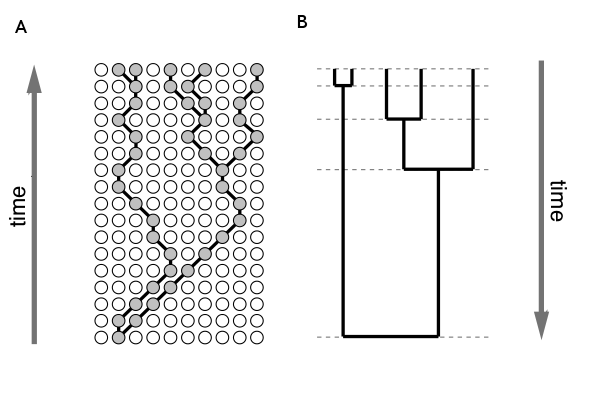
\includegraphics[scale=0.4]{wright-fisher} 
\caption{
{ \footnotesize 
{\bf The Wright-Fisher population model and Kingman's $n$-coalescent} A. A Wright-Fisher population of $N=10$ individuals. The lineages for all individuals sampled from the population coalesce to a common ancestor.
B.  In Kingman's $n$-coalescent, time is continuous and measured from tips towards the root.
}% END: footnotesize
}
\label{fig:wright-fisher}
\end{figure}

Under the Wright-Fisher model, the population size $N$ is assumed to be constant through time.
Time (generations) is discrete, i.e. every individual is replaced in every generation, with all individuals having equal chances of reproducing.
To understand how we can describe the coalescent process for a small sample of individuals from such populations as a function of their size, let us start with numbering time (generations), starting from present one as $t_{0},t_{1},t_{2},\ldots,t_{k}$.
The probability that two individuals sampled at the present generation $t_{0}$ share a common ancestor at a preceding generation $t_{1}$ is $\frac{1}{N}$.
The probability that two individuals sampled at $t_{0}$ share an ancestor at $t_{2}$ is the probability that they do not share an ancestor at $t_{1}$, which is $1-\frac{1}{N}$, times the probability of sharing an ancestor at $t_{2}$, which is $\frac{1}{N}$, as the population size remains constant every generation.

%\begin{remark}{Sir John Frank Charles Kingman}
%\begin{figure}[H]
%\centering
%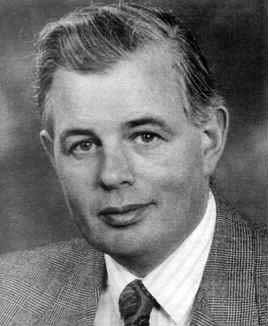
\includegraphics[scale=0.4]{kingman} 
%\caption{
%{ \footnotesize 
%% {\bf Sir John Frank Charles Kingman.} 
%This suave looking gentleman is a British mathematician, with his most notable work on the mathematics of the coalescent, a process fundamental to modern population genetics. 
%Interestingly Kingman never completed his PhD.
%}% END: footnotesize
%}
%\label{fig:kingman}
%\end{figure}
%\end{remark}

Generalizing this, we can write down the probability that a pair of randomly sampled individuals will have their most-recent common ancestor (MRCA) at time $t_{k}$:

\begin{equation}
P\left(t_{k}\right)=\left(\frac{1}{N}\right)\left(1-\frac{1}{N}\right)^{k-1}.
\label{eq:wright-fisher-two-individuals}
\end{equation}

\noindent
Now instead of sampling just two individuals we sample $n,\;2<n\leq N$ individuals, where $n\ll N$.
There are now $\frac{n\left(n-1\right)}{2}$ pairs in $t_{0}$ which can coalesce in $t_{1}$ and each pair has  $\frac{1}{N}$ probability of sharing the same ancestor, therefore:

\begin{equation}
P\left(t_{1}\right)=\frac{n\left(n-1\right)}{2N}.
\label{eq:wright-fisher-n-individuals}
\end{equation}

\noindent
Similarly as in the case of a pair of individuals we can generalize Equation~\ref{eq:wright-fisher-n-individuals} and write down the probability that the sampled pairs of individuals coalesce at $t_{k}$:

\begin{equation}
P\left(t_{k}\right)=\left(\frac{n\left(n-1\right)}{2N}\right)\left(1-\frac{n\left(n-1\right)}{2N}\right)^{k-1}.
\label{eq:wright-fisher-n-individuals-general}
\end{equation}

\noindent
Equation~\ref{eq:wright-fisher-n-individuals-general} characterizes a probability mass function (PMF) of a geometric distribution with parameter $p=\frac{n\left(n-1\right)}{2N}$ (see Equation~\ref{eq:geometric_dist}).

\begin{remark}{Geometric distribution}
The geometric distribution returns the probability that the $k$-th trial out of $k$ independent Bernoulli trials, each with success probability $p$, is a successful one:

\begin{equation}
P\left(X=k\right)=p\left(1-p\right)^{k-1},\;0<p\leq1,\; k\in\left\{ 1,2,3,\ldots\right\}.
\label{eq:geometric_dist}
\end{equation}

\noindent
Cumulative distribution function of the geometric distribution:
\begin{equation}
P(X\leq k)=1-\left(1-p\right)^{k-1}.
\label{eq:geometric_cdf}
\end{equation}
\end{remark}

For small values of $p$ the discrete geometric distribution can be approximated by its continuous equivalent, the exponential distribution. 
%An informal argument finds itself in Figure~\ref{fig:exp_approx}.
%
%\begin{figure}[H]
%\centering
%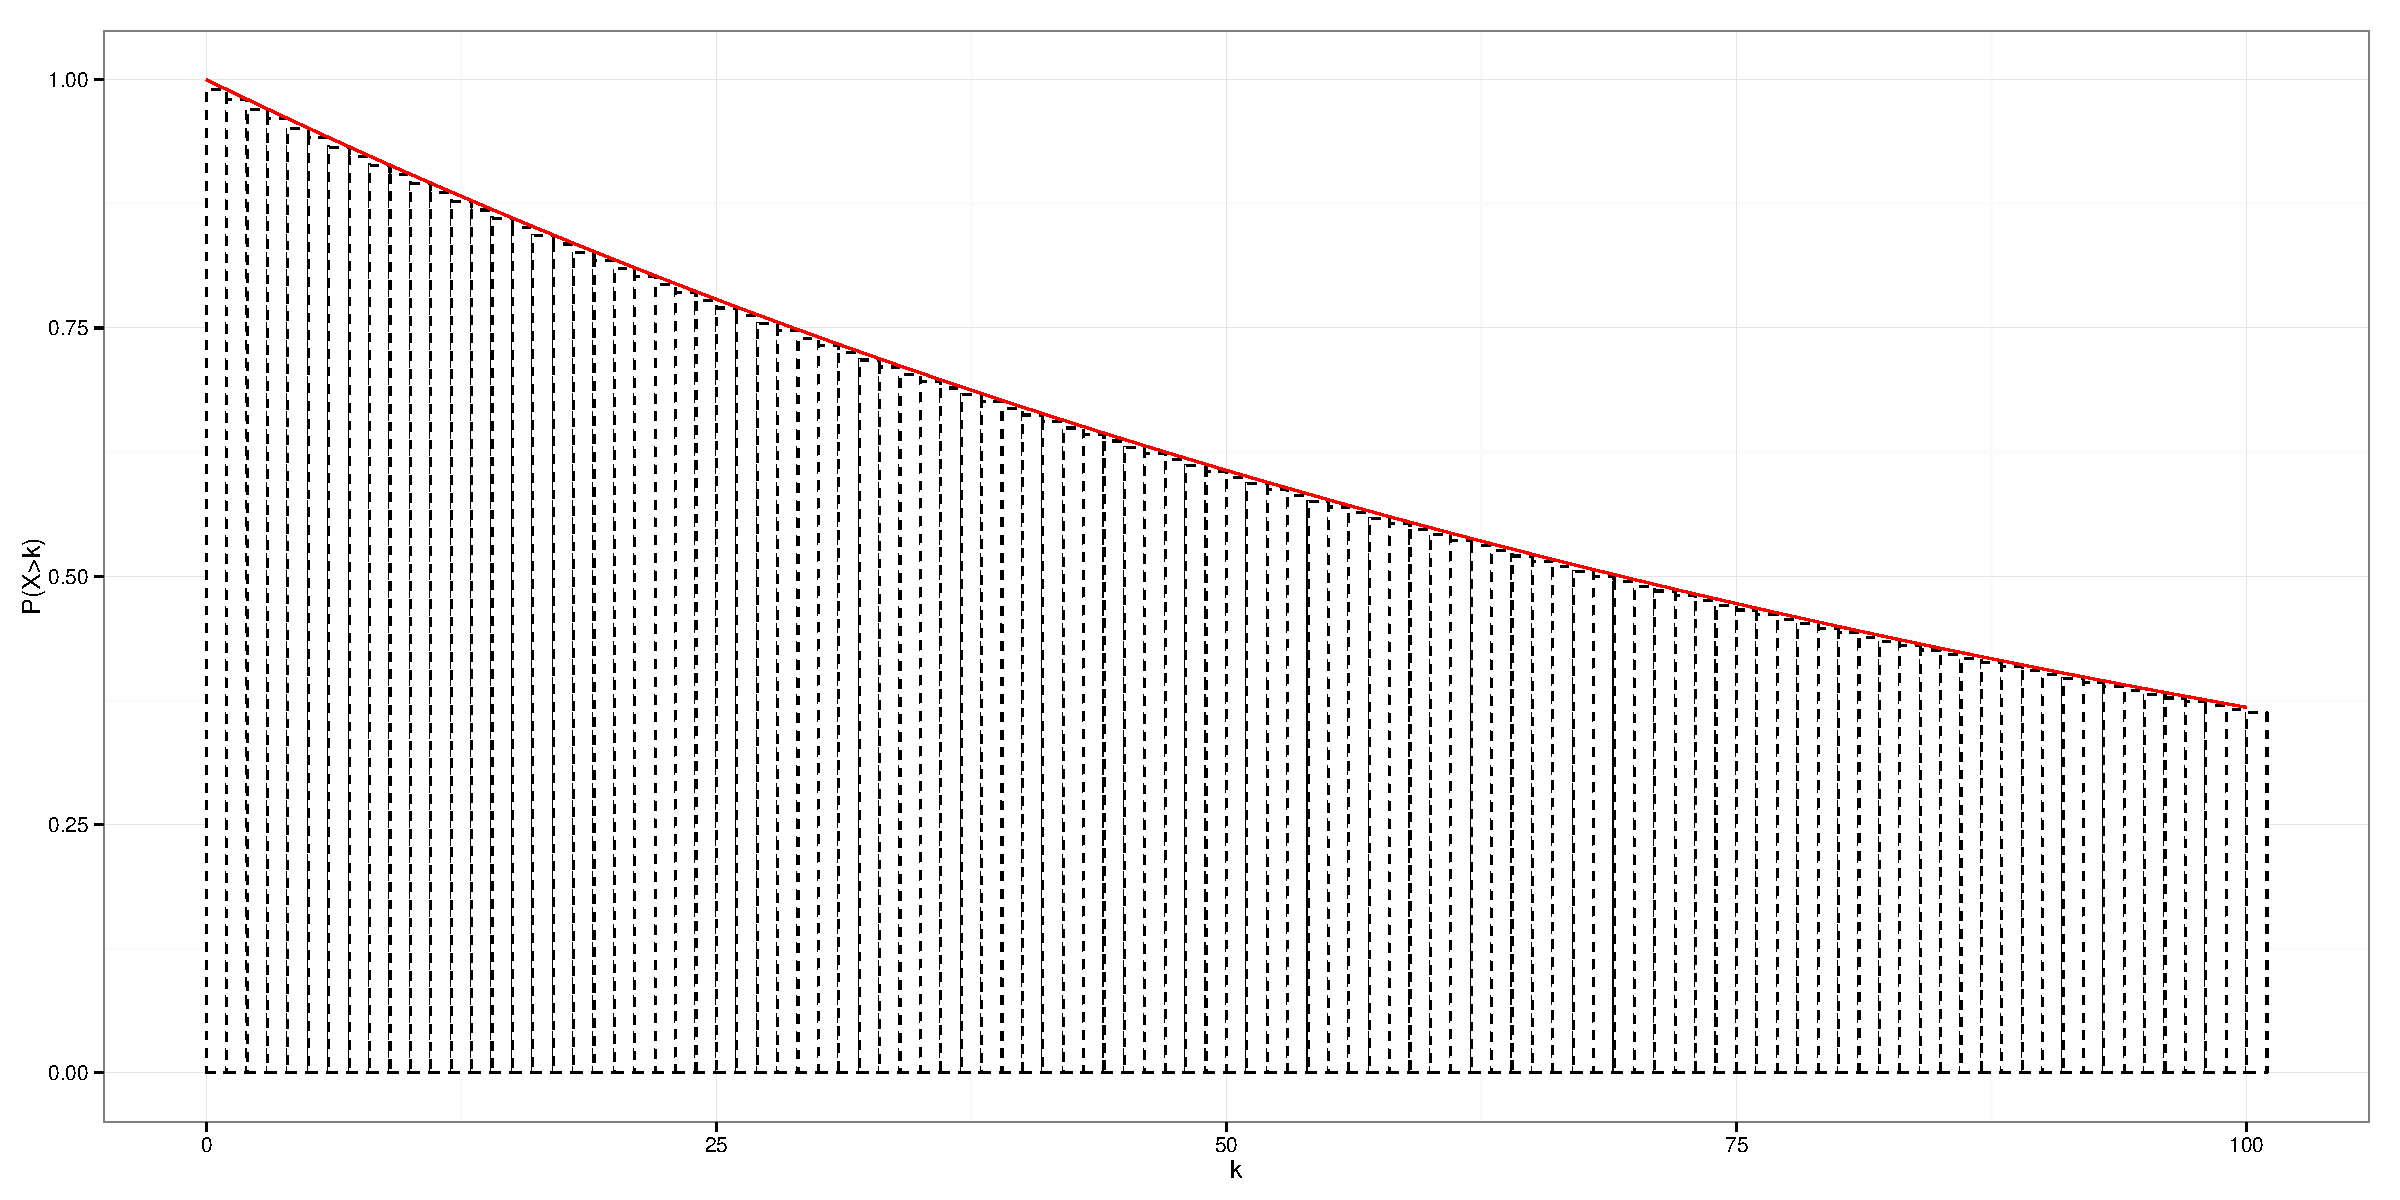
\includegraphics[scale=0.3]{exponential_approx} 
%\caption{
%{ \footnotesize 
%{\bf Approximating geometric distribution by exponential distribution.} 
%Black rectangles denote the discrete geometric distribution, red line is the continuous geometric distribution.
%}% END: footnotesize
%}
%\label{fig:exp_approx}
%\end{figure}
%
This approximation allows us to move into continuous time, and we can write Equation~\ref{eq:wright-fisher-n-individuals-general} as:

\begin{equation}
P\left(t_{k}\right)=\frac{n\left(n-1\right)}{2N}\textrm{exp}\left(-\frac{n\left(n-1\right)}{2N}k\right)
\label{eq:exponential_time}
\end{equation}

In the light of Equation~\ref{eq:exponential_time} we consider Kingman's coalescent as a continuous time version of the Wright-Fisher model with $n$ sampled individuals.
\cite{Rodrigo1999} developed an extension of Kingman's coalescent, the so-called \textit{serial coalescent} (s-coalescent), that allows to scale the genealogies in real time units.
Genealogies for a small sample of individuals can be estimated from their genetic data using phylogenetic reconstruction, and the resulting waiting time distributions in the trees can be used to estimate population sizes.
It is important to note, however, that these models make assumptions that are clearly violated in most populations and therefore lead to population size estimates that generally  deviate strongly from census population sizes. 
In order to still be able to use those models, a rescaling of the population model has been proposed so that it behaves, with regard to certain properties, as a simple Wright-Fisher model with constant population size.
This rescaling requires moving from census population size to the more abstract concept of `effective population size' or $N_{e}$.

As changes $N_{e}$ still reflect changes in the census population, the constant population size coalescent model has been extended to account for variable size populations, either in parametric \citep{Pybus2002} or non-parametric formulations \citep{Minin2008, Gill2013}. 
In a Bayesian framework focusing on time-measured trees, such process models find their use as priors on trees.
Coalescent models have also been extended to account for structured populations allowing to estimate migration rates, which naturally brings us to spatial dynamics \citep{Kuhner2006,migrate}.

% Introduce phylogeography
How geography impacts genealogies is one the main research questions of phylogeography, a discipline that frequently resorts to ancestral reconstruction to shed light on migration or dispersal dynamics. 
%Another process which shapes the phylodynamics of viral sequences is the process of their migration, which we understand as a dispersal in actual geographical coordinates.  
%Inference methods which make use of both molecular and geographical data have been dubbed as phylogeography as the processes which shape the genome are integrated with the processes of geographical spread.
In that sense, the inferred tree does not only provide a record of evolutionary ancestry, but also of the dispersal process that gave rise to the current geographic distribution of taxa.
%
%% snow
%Perhaps a first know study which used epidemiological methods which we today call phylodynamics, is the famous John Snow's work in 1854, tracing the source of a cholera epidemic in the Soho district of London.
%There was no notion of molecular data or even bacteria nor viruses, yet by using a dot map Snow was able to show that almost all the cases in were clustered in a close proximity of a water pump on the Broad Street (see Figure~\ref{fig:snow}).
%Snow was able to persuade local authorities to remove the handle, which contributed to the end of the outbreak.
%It was later found that a nearby cesspool was in fact leaking its content into the public well, therefore transmitting water contaminated with the cholera bacteria.
%
%\begin{figure}[H]
%\centering
%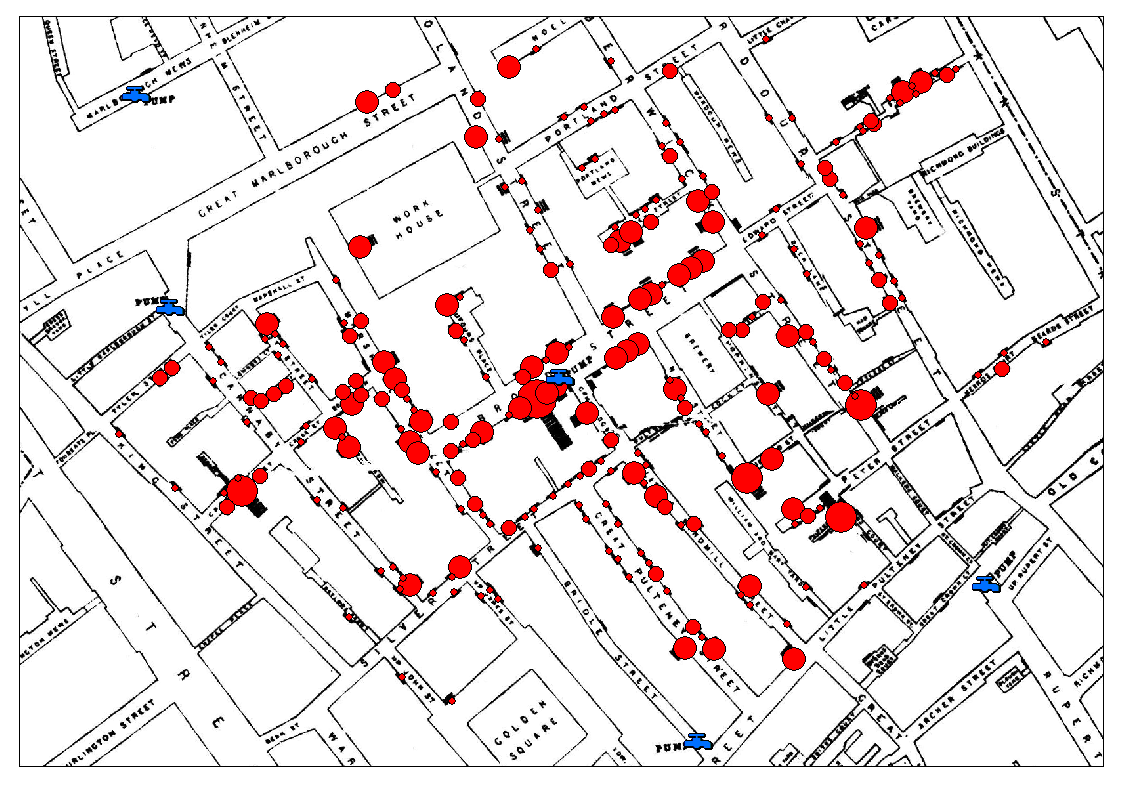
\includegraphics[scale=0.4]{snow_map} 
%\caption{
%{ \footnotesize 
%{\bf Map of the cholera cases in the London epidemic of 1854.} 
%Map shows the clustering of cases around water pump on the Broad Street (currently called Broadwick Street).
%}% END: footnotesize
%}
%\label{fig:snow}
%\end{figure}
%
% stochastic model based
In their opinion piece on current methods in phylogeography, \cite{Bloomquist2010} highlight fully probabilistic approaches that use Continuous-time Markov chain (CTMC) models to infer transitions between discrete locations as a function of continuous time as one of the phylogeographic inference methods.
Maximum likelihood and closely related Bayesian inference methods assume that both evolution and geographical dispersal are independent, stochastic processes which unfold on phylogenetic trees.
\cite{Lemey2009} and \cite{Lemey2010} developed a Bayesian framework that allows for a joint reconstruction of spatial diffusion and genetic ancestry, accommodating important sources of uncertainty in estimating spatial and temporal dynamics.
Because they are both modeled using CTMCs, the work presented here on CTMC model extensions finds applications to sequence evolutionary processes as well as these phylogeographic processes.

% population genetic / migration models
%The coalescent which we described at the beginning of this Subsection, and more generally population genetic approaches are another statistical inference method that can be naturally extended for phylogeography.
%These methods assume that trees are shaped by processes such as migration, selection or fluctuations in the population sizes in time.
%Trees proposed by the coalescent are then random draws from a larger, population-level processes, and one can use molecular and other data to get a better resolution of these underlying processes.

\subsection{Bayesian evolutionary inference in BEAST}

The Bayesian evolutionary analysis by sampling trees (BEAST) software \citep{Drummond2012}, to which our research group contributes, integrates many of the advances described in Subsections~\ref{sub:epidemiology}-\ref{sub:molecular_clock}.
BEAST is set in a Bayesian statistical framework, meaning that it combines the data likelihood (see Subsection~\ref{sub:likelihood}) with prior knowledge (see Section~\ref{sec:bayesian_inference}), and generates posterior samples using MCMC (see Subsection~\ref{sub:mcmc}).

% other packages
BEAST is not the only software package for Bayesian phylogenetic analysis and can be compared to a number of other packages.
MrBayes \citep{Huelsenbeck2001} is a command-line driven software mainly focusing on phylogenetic inference.
Migrate-n \citep{migrate} and LAMARC \citep{Kuhner2006} on the other hand concentrate on coalescent-driven population genetics.
At the core of BEAST lies a Metropolis-Hasting algorithm (\cite{Metropolis1953, Hasting1970}, see also Subsection~\ref{sub:mcmc}) for constructing Markov chains that converge on the posterior distribution as the equilibrium distribution.
This is precisely why BEAST is not meant for reconstructing a single tree or a point estimate for a parameter of interest, but rather generates samples that can be used to summarize distributions of mutation rates, divergence times, demographic parameters, trait evolution or others.

%beast
Compared to other similar programs, BEAST stands out in the number of models available for performing inference and the flexibility by which they can be combined.
Perhaps the most characteristic point is that BEAST uniquely focuses on sampling rooted, time-measured phylogenies.
This allows for a very natural interpretation of reconstructed trees, and is achieved thanks to the adoption of molecular clock models, from a simple strict clock model, with an equal rate across the whole time-span of the evolution, to relaxed molecular clock models that model rate variation in various ways \citep{Thorne1998,Yoder2000,Drummond2006,Drummond2010}.
BEAST offers a large number of complementary evolutionary models, which can be combined in a flexible way.
Various substitution models for performing analysis on nucleotide, codon or amino-acid data, accounting for among-site and among-lineage rate variation and partitioned in arbitrary ways, are complemented with demographic tree priors such as coalescent \citep{Drummond2005,Minin2008b} or birth-death priors \citep{Nowak2006} and trait evolutionary models.

% using beast
%The program takes as input structured XML files which describe the data to be analyzed, the models to be used, the number of samples to collect from the posterior and the output options.
%The output consists of a simple tab-separated files, with each row corresponding to one value sampled from the posterior distribution, for both the parameter values and actual trees.

%gpus
\myedit{DPfive}{
% The growing availability of large complex data-sets has led to the term `Big Data'. %being coined.
% Large sample sizes, such as full genome sequences or the ones generated with next-generation sequencing techniques are increasingly challenging phylogenetic inference.
Growing availability of large sample size, complex data-sets such as full genome sequences or the ones generated with next-generation sequencing techniques are increasingly challenging phylogenetic inference.
}%END: myedit
Fortunately strategies have been proposed to reduce the time that it takes to fit complex phylogenetic models to vast amounts of data.
These solutions are mainly focused on parallellization and on harnessing the capabilities of modern graphics processing units (GPUs), such as the NVIDIAs Tesla line of GPUs that target the high performance computing market.
BEAGLE (Broad-platform evolutionary analysis generalized likelihood evaluator, \cite{Ayres2012}), is a library that can be used in conjunction with BEAST and provides an API (Application Programming Interface) that massively parallel graphics processors and other multicore devices can exploit to substantially decrease the runtime of phylogenetic analysis \citep{Suchard2009}.
%BEAST readily integrates with BEAGLE and provides a GUI interface to configure the library.

% external software
BEAST is packaged with a number of additional utilities that can either assist in generating the input for BEAST, in analyzing the results or in some other specific tasks.
\textbf{BEAUti} (Bayesian Evolutionary Analysis Utility) is a  GUI (graphical user-interface) application for generating XML input files for BEAST. 
% It alleviates some of the most cumbersome tasks that would otherwise have to be done manually, thus saving time and simplifying 
It supports the specification of (standard) models, priors, operators, and MCMC chain settings, without having to resort to a manual editing of the XML syntax.
\textbf{LogCombiner} combines log files from multiple runs, that can then be imported into \textbf{Tracer}, a graphical tool for the analysis and visualization of the output of BEAST as well as other common MCMC packages.
It allows for a quick inspection of mixing, convergence, and summary statistics of the parameters of interest.
\textbf{TreeAnnotator} summarizes the tree log files and generally represents the evolutionary history using a maximum clade credibility (MCC) tree; each node or branch in this tree can be annotated with external information, such as posterior probabilities and maximum a posteriori ancestral traits.
The tree and its annotated information can subsequently be visualized using \textbf{FigTree} (\url{http://tree.bio.ed.ac.uk/software/figtree/}). % or if nodes of the trees are annotated with spatial information they can be displayes in geographical coordinates using \textbf{SPREAD}. %PL we need to introduce spread first, which is a chapter in this thesis :-), same for piBUSS
%Finally \textbf{$\pi$BUSS} is a software for sequence simulation, capable of generating XML files understood by BEAST for combined simulation-inference analysis as well as sequences in formats taht can be imported into any other phylogenetic software.
%
In conclusion, BEAST is a flexible package for statistical pylogenetics and hypothesis testing.
The software is continuously being improved and new models are being developed, but the development has recently been split into a continuing BEAST1 branch and a new BEAST2 branch\citep{Bouckaert2014}. 
Since the work presented in this thesis is implemented in BEAST1, all references to BEAST will implicitly refer to this development branch.
%In addition to a large array of available models, it is actively developed with new models and enhancements included with every new stable release.

\subsection{Objectives: model extension, simulation and visualisation\label{sub:objectives}}

% models
\paragraph{}
Phylogenetic analyses employing stochastic processes make strong restrictive assumptions regarding the underlying substitution process.
These assumptions are mainly enforced to reduce the number of free parameters of the models and to ease computational and mathematical tractability.
Unfortunately, many of these assumptions hamper the application of the methods to complex, real-world data sets.
Relaxing some of these assumptions and developing more biologically plausible models, able to grasp the complex nature of phylodynamic dispersal processes is an important aim of this thesis \citep{Bielejec2014a}.
%Another goal is to make the general applicability suitable for epidemiological problems as well as beyond them, with potential to turn the findings into useful predictions of the emergence of infectious diseases, e.g. by identifying the sources and sinks of the viral spread.
% geographical dispersal

% simulation
\paragraph{}
The development of novel phylogenetic inference methods brings about the need to compare estimator performance and to characterize strengths and weaknesses of different approaches (e.g. \cite{Arenas2012}, \cite{Hoban2011}).
Whereas the true underlying evolutionary relationships between biological sequences are generally unknown, Monte Carlo simulations allow to generate test scenarios while controlling the evolutionary history as well as the tempo and mode of evolution. 
Part of the research presented in this thesis is devoted to the development of flexible software for sequence simulation, that integrates both the tree-generative processes, as well as models responsible for shaping the molecular histories and geographical dispersal \citep{Bielejec2014a}.

% visualisation
\paragraph{}
Bayesian phylogenetic inference inevitably results in complex, multi-dimensional output.
Adding the geography to the phylogenetic process further adds to this complexity.
In particular, Bayesian phylogeography results in posterior distributions of trees, with each tree branch annotated with estimated node locations and other traits of interest.
%This represents a major challenge for visualization  the phylogenetic inference.
Clear and intuitive visualizations are an important aspect of every analysis \citep{Hadley2010}, but this is far from trivial for the estimates resulting from Bayesian analysis of sequences and traits.

Spatial phylogenetic projections have already been utilized in the field \citep{Kidd2006,Parks2009}, yet most of these applications remain limited to mapping phylogenetic tip taxa to their geographical coordinates, without providing robust statistical estimates of the geographic locations at the ancestral nodes nor the measures of uncertainty in the inference.
Fortunately, the advent of powerful and flexible Geographic Information Systems (GIS) has fostered an interesting possibility to visualize both the spatial and temporal information resulting from viral phylogenetic analysis.
Presenting readily interpretable visual summaries of the inferences that can be communicated to the researchers across different fields is one of the more important aspects of this thesis.

\section{Evolution as a stochastic process\label{sec:markov}}

In order to provide a formal basis for the work in the research chapters of this thesis, this chapter proceeds with a description of general stochastic models of character substitution processes in phylogenetics. 
Molecular phylogenetic modeling typically starts with an assumption that the observed sequence data has been generated by some stochastic process, which emits characters over time.
We can think of these stochastic processes as functions of time, which is regarded as a deterministic argument, whose values are random (non-deterministic) variables. 
It is thus a statistical model of a random development, or evolution, in time.
Phylogenetic inference often resorts to processes where time is considered to be continuous and the indexed set of outcomes, called the state space, is countable and finite (discrete).
With that in mind we can provide a formal definition:

\begin{definition} 
The stochastic process $X$ is a collection $\left\{ X(t):\; t\in T\right\} $, where each drawn value $X(t)$ is a random variable drawn from state space $\mathcal{E}$, with $K$ possible values, indexed by orderer time $T$.
\label{def:stochasticProc}
\end{definition} 

In the simplest case, for which the unit of evolution is a single nucleotide, we have $\mathcal{E}=\left\{ A,C,G,T\right\}$ and $K=4$.
%GB: perhaps point out that they're in fact not independent?
The particular sites of the sequence alignment are then considered to be stochastically independent realizations of the process $X$, leading to the observed data (see Figure~\ref{fig:alignment}). 


%PL: Since you list the mutations for the right branch, you may as well list the one on the left branch as well
% FB: not sure what you mean, should I add some annotation on that branch? I explicite left it empty, the right branch is longer so it has more substitutions on it than the left one
\begin{figure}[h!]
\centering
\begingroup
\everymath{\displaystyle}
{\Large
\begin{displaymath} % 
\xymatrix{
& \color{gray2}A \ar[dl] \ar[drdr]^{ \color{gray2}\begin{array}{c}
A\rightarrow G\\
G\rightarrow C
\end{array}} & & \\
T & & & \\
& & & C \\
}
%     \xymatrix@R+1pc{ 
% \color{gray2}A \ar[r] & \color{gray2}T \ar[r] & A \\
% \color{gray2}A \ar[r] & \color{gray2}T \ar[r] & G \\
% \color{gray2}A  \ar[rr]_{ \color{gray2}\begin{array}{c}
% A\rightarrow G\\
% G\rightarrow C
% \end{array}} &&  C
%     } % 
\end{displaymath}
}% END: Large
\endgroup
\caption{
{ \footnotesize 
{\bf Evolution at a single site.} Over time characters at the site change, leading to the observed data (black). 
%Some of the mutations may be unobserved. %PL: All mutations are unobserved!!!!
Each site evolves independently.
The longer the evolutionary time, the higher the probability that multiple substitutions occur on the same site.
}% END: footnotesize
}
\label{fig:alignment}
\end{figure}

As illustrated in Figure~\ref{fig:alignment}, multiple substitutions (multiple hits) may occur, which complicates the estimation of the underlying evolutionary distances from the observed data.
Specifically, the number of observed differences in the sampled genetic data will be an underestimate of the underlying genetic distance (in Figure~\ref{fig:alignment}, three substitutions underlie a single difference in the observed states).
In order to accurately describe these processes, one needs a model of evolution that can account for those multiple hits.

\subsection{The Poisson process\label{sub:poisson}}

The Poisson process is an example of a continuous-time stochastic process that is frequently used to describe counts of independent, rare events, occurring with some intensity (or rate) $r$, that remains constant over time. 
Examples of such a process are the requests for a single document on a web-server, or the goals scored in a football game \footnote{Unless it's Real - Barca, than the events are not so rare.}. %PL or Brazil - Germany...
%The state space in this case is obviously $\mathcal{E} = \left\{ 0,1,2, \dots \right\}$.
The Poisson process is equally suitable to model the number and waiting times of DNA mutation of sequence substitution events. 
We can formally define a Poisson process as following:

\begin{definition} 
A Poisson process with rate $r>0$ is a continuous-time counting process $\left\{ N(t):\; t\geq0\right\}$ such that:

\begin{itemize}
\item $N(0)=0$.
\item The increments are independent i.e. if $(t_{1},t_{2}]\cap(t_{3},t_{4}]=\emptyset$ then $N(t_2)-N(t_1)$ and $N(t_4)-N(t_3)$ are independent and stationary (i.e. the probability distribution of the number of occurrences counted in any time interval only depends on the length of that interval).
\item The number of events in any interval of length $t$ is $\text{Poisson}(r t)$.
\end{itemize}

\label{def:poisson}
\end{definition}

Figure~\ref{fig:poisson} shows a sample of different trajectories for such a process.

\begin{figure}[h!]
\centering
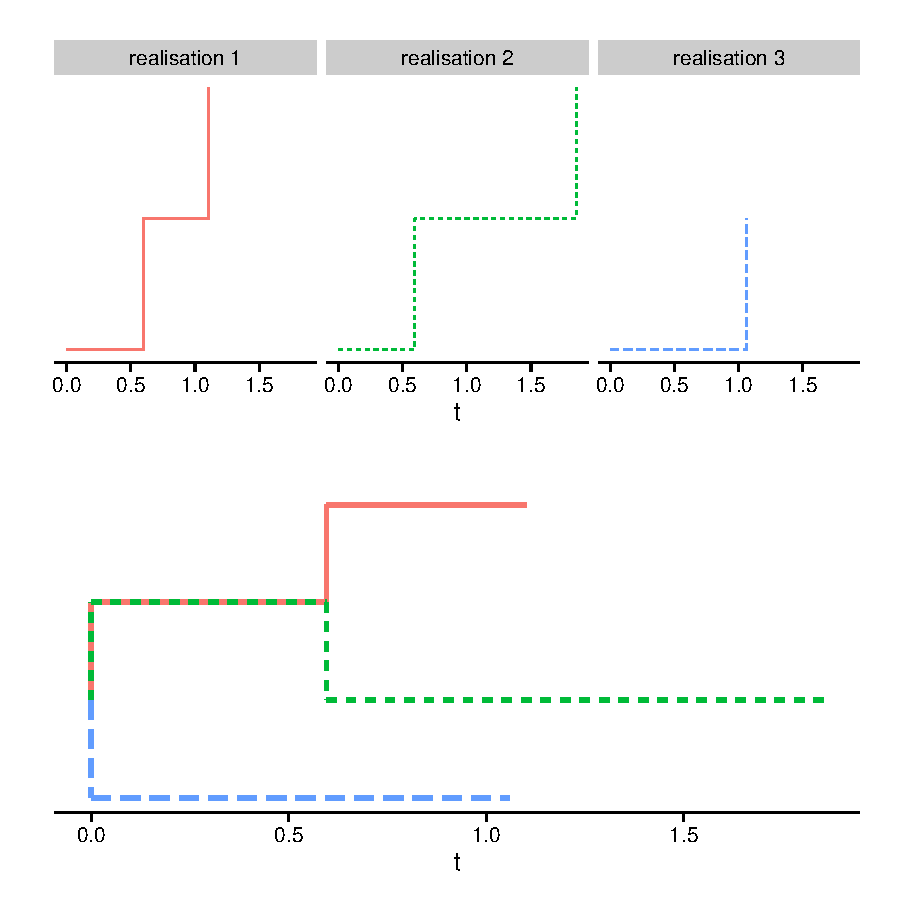
\includegraphics[scale=0.4]{poisson}
\caption{
{ \footnotesize 
{\bf Three independent realizations of the Poisson process with intensity $r=1$.}
Waiting times between mutations are \emph{iid} exponentially distributed random variables with mean $1/r$.
} % END: footnotesize
}
\label{fig:poisson}
\end{figure}

Let's assume that evolution at a single site is governed by a Poisson process $N$ with some intensity $r$.
Definition~\ref{def:poisson} implies that under this model the number of mutations $N(t+u)-N(u)$ in some time interval $(u,t+u]$ of length $t$ follows a Poisson distribution with expected number of events $r t$.
Thus we can write:

\newpage

\begin{align}
P\left\{ N(t+u)-N(u)=k\right\} & = P\left\{ N(t)=k\right\} \nonumber \\
= \frac{e^{-r t}(r t)^{k}}{k!},\; k=0,1,\ldots
\label{eq:poissonDist} 
\end{align}

In the Poisson process the time between any two mutations is exponentially distributed with parameter $r$, thus the average waiting time between the occurrence of events is $1/r$.
To show this important property we can consider $T_1,T_2,\ldots$ to be the inter-arrival times, where $T_k$ is the waiting time between the $(k-1)\text{'st}$ and $k\text{'th}$ mutation. 
Obviously, the number of mutations before some time $t>0$ is less than some integer $k>0$ if and only if the waiting time $T_k$ until the $k\text{'th}$ mutation is larger than $t$:

\begin{equation}
P\left(N(t)<k\right)=P\left(T_{k}>t\right).
\end{equation}

\noindent
For the first waiting time $T_1$ we have:

\begin{equation}
1-P\left(T_{1}>t\right)=1-P\left(N(t)<1\right)=1-P\left(N(t)=0\right).
\end{equation}

\noindent
From Equation~(\ref{eq:poissonDist}) we have that:

\begin{equation}
F_{T_{1}}(t)=1-P\left(T_{1}>t\right)=1-e^{-r t}.
\end{equation}

\noindent
$T_1$ therefore follows the exponential distribution with parameter $r$.
For the second waiting time $T_2$ and some arbitrary $u>0$ and $t>0$, the independent increments property implies that:

\begin{eqnarray}
F_{T_{2}}(t) &=& 1-P\left(T_{2}>t|T_{1}=u\right) \nonumber \\
& = & 1-P\left(\text{no mutations in }(u,t+u]|T_{1}=u\right) \nonumber \\ 
& = & 1-P\left(N(t)=0\right)=1-e^{-r t}.
\end{eqnarray}

\noindent
Therefore, $T_2$ is independent of $T_1$ and $\text{Exponential}(r)$ distributed. 
Similarly we can show that $T_3$ is independent of $T_1$ and $T_2$ and by repeating the same argument: $T_1,T_2,\ldots$ are independent and identically distributed (i.i.d.) $\text{exponential}(r)$ random variables.

% TODO: memoryless property does not depend at all, vide poiss)
% TODO: markovian (depends only a little)
% * difference? Memoryless is more

\subsection{Instantaneous rates of mutation\label{sub:rates}}

Within a phylogenetic framework the interest typically lies not only in modeling the number of events (mutations), but also the actual probabilities of changing states at the particular site in the alignment. 
We therefore need to generalize the process to a finite number of discrete states.
Let $\mathbf{R}$ denote a $K \times K$ matrix filled with probabilities of exchanging states between any pair $i,j\in \mathcal{E}$.
To express the probability of going from state $i$ to $j$ in some time interval $t$, we multiply the probability of the state change by the probability of having exactly $k$ events leading to the observed change, and integrate over all possible values of $k$.
This allows us to accommodate all possible paths that evolution might have taken, and to account for multiple hits that might have occurred at the site, as illustrated in Figure~\ref{fig:alignment}.
From Equation~(\ref{eq:poissonDist}) we know the probability of having $k$ mutations in time interval $t$, thus:

\begin{equation}
\left\{ P(t) \right\} _{ij}= \left\{ \underset{k=0}{\overset{\infty}{\sum}}\mathbf{R}^{k}\frac{(r t)^{k}}{k!}e^{-r t} \right\} _{ij} = \left\{ \underset{k=0}{\overset{\infty}{\sum}}\frac{(\mathbf{R}r t)^{k}}{k!}e^{-r t} \right\} _{ij},
\label{eq:matrixExp1}
\end{equation}

\noindent
where $\left\{  \cdot \right\} _{ij}$ denotes the $ij\text{-th}$ element of a matrix.
% the transition probability matrix $\mathbf{P}$ over time $t \geq 0$.
Let us denote the matrix $\mathbf{R}-\mathbf{I}$, where $\mathbf{I}$ is a $K \times K$ identity matrix, by $\mathbf{Q}$.
Using the power series definition of the transition probability matrix: $\exp(\mathbf{R})=\underset{k=0}{\overset{\infty}{\sum}}\mathbf{R}^{k}/k!$, we can write Equation~(\ref{eq:matrixExp1}) as:

\begin{equation}
\left\{ \left\{ P(t)\right\} _{ij} \right\} _{ij} = \left\{ e^{\mathbf{R}r t}e^{-r t} \right\} _{ij} = \left\{ e^{(\mathbf{R}-\mathbf{I})r t} \right\} _{ij}= \left\{ e^{\mathbf{Q}r t} \right\} _{ij}
\label{eq:matrixExp2}
\end{equation}

\noindent
A single entry $q_{ij} \ge 0$ for $i \neq j$ in matrix $\mathbf{Q}$ quantifies the probability of changing from state $i$ to $j$ in an infinitely small amount of time, therefore we will refer to $\mathbf{Q}$ as the \emph{instantaneous rate matrix}.

\subsection{Computing the matrix exponent \label{sub:exponentiation}}

In order to arrive at the finite-time transition probability matrix $\mathbf{P}(t)$ for some time $t\geq0$, one needs to compute the matrix exponential in Equation~\ref{eq:matrixExp2}.
\cite{Moler1978} provide an excellent review of numerical methods to compute the matrix exponent. 
Here, we highlight the method utilized by most phylogenetic software, including BEAGLE \citep{Ayres2012} and BEAST \citep{Drummond2012}, that uses the singular value decomposition (SVD) of the rate matrix $\mathbf{Q}$.   

Let us assume $\mathbf{Q}$ has $K$ linearly independent eigenvectors $\mathbf{v}_{i} \; (i=1,\ldots,K)$ with corresponding eigenvalues $\lambda_{i}\;(i=1,\ldots,K)$:

\begin{equation}
\mathbf{Q}\times\mathbf{V}=\lambda\times\mathbf{V}
\label{eq:eigenvaluesEigenvectors}
\end{equation}

\noindent
This condition is sufficient for $\mathbf{Q}$ to be diagonizable, thus its Jordan form is:

\begin{align}
\mathbf{V}\times\mathbf{Q}\times\mathbf{V}^{-1}=\left[\begin{array}{cccc}
\lambda_{1} & 0 & \cdots & 0\\
0 & \lambda_{2} & \ddots & \vdots\\
\vdots & \ddots & \ddots & 0\\
0 & \cdots & 0 & \lambda_{K}
\end{array}\right] %\nonumber \\
= \text{diag}(\lambda_{1},\ldots,\lambda_{K})=\mathbf{D} ,
\label{eq:diagonalization}
\end{align}

\noindent where $\mathbf{V}$ is a matrix composed of eigenvectors of $\mathbf{Q}$. 
Multiplying both sides of Equation~(\ref{eq:diagonalization}) with the edge length $t$ and scaling by the appropriate rate scalar $r$, we can write $\mathbf{Q}$ in the following form:

\begin{equation}
rt\mathbf{Q}=\mathbf{V}\times\text{diag}(rt\lambda_{1},\ldots,rt\lambda_{K})\times\mathbf{V}^{-1} .
\end{equation}

\noindent Finally, using the power series definition of the transition probability matrix, we obtain: 

\begin{align}
\mathbf{P}(t) & =  \exp\left(rt\mathbf{Q}\right) \nonumber \\
& =   \underset{k=0}{\overset{\infty}{\sum}}\left(rt\mathbf{Q}\right)^{k}/k! \underset{k=0}{\overset{\infty}{\sum}}\left(\mathbf{V}\times\mathbf{D}\times\mathbf{V}^{-1}\right)^{k}/k! \nonumber \\
& =  \mathbf{V}\times\left(\underset{k=0}{\overset{\infty}{\sum}}\mathbf{D}^{k}/k!\right)\times\mathbf{V}^{-1} \nonumber \\
& =  \mathbf{V}\times\text{diag}(e^{rt\lambda_{1}},\ldots,e^{rt\lambda_{K}})\times\mathbf{V}^{-1} ,
\label{eq:eigen_decomposition}
\end{align}

\noindent 
where the last transition is due to the fact that the exponential of the diagonal matrix is obtained by exponentiating every entry on the main diagonal.
We should note here that the repeated evaluations of $\exp\left(rt\mathbf{Q}\right)$ for different times $t$ are all based on the same SVD of the matrix $\mathbf{Q}$. 
One needs only to scale and exponentiate the eigenvalues to calculate the diagonal matrix $D$ and perform two matrix multiplications, thus reducing all calculations to a simple and effective algorithm. 

\subsection{Markov chain models of sequence substitution\label{sub:subst_models}}

After obtaining finite-time transition probabilities given by Equation~\ref{eq:eigen_decomposition} for some time $t\geq0$ one can start drawing realizations, which follow probabilities defined by $\mathbf{P}$.
These realizations constitute a continuous-time stochastic process $\left\{ X(t):\; t\geq0\right\}$, which inherits the Markov property from the Poisson process modelling the time between any two mutations, as defined in Subsection~\ref{sub:poisson}.

We say that a stochastic process has the Markov property if the conditional probability distribution of future states of the process depends only upon the present state, not on the sequence of events that preceded it, i.e. for every $n\geq 0$, given the time points $0\leq t_{0}\leq t_{1}<\ldots<t_{n}\leq t_{n+1}$ and discrete states $i_{0},i_{1}, \ldots, i_{n},i_{n+1}$, it holds that: 

\begin{align}
& P\left\{ X(t_{n+1}) = i_{n+1}\mid X(t_{n})=i_{n},\ldots, X(t_{0})=i_{0}\right\}   \nonumber \\
&= P\left\{ X(t_{n+1}) = i_{n+1}\mid X(t_{n})=i_{n}\right\} .
\label{eq:markov}
\end{align}

The elements of $\mathbf{P}$ quantify the finite-time transition probabilities between the $K$ discrete state-space elements.
This describes a Continuous-time Markov chain (CTMC), which  we will use to model the substitution process at a single site of an alignment.
Every CTMC is completely characterized by its rate matrix $\mathbf{Q}$ and the stochastic matrix $\mathbf{P}(t),\ t\geq0$ is obtained via matrix exponentiation as described in the previous subsection (Subsection~\ref{sub:exponentiation}).

%---SUBSTITUTION MODEL---%
\begin{figure}[h!]
\centering
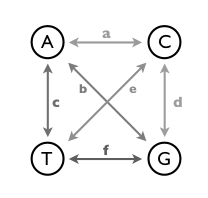
\includegraphics[scale=0.5]{substitution} 
\caption{
{ \footnotesize 
{\bf  Graphical representation of a nucleotide substitution model.} 
Markov substitution model with 6 parameters describing the symmetric transition rates.
} % END: footnotesize
}
\label{fig:substitution}
\end{figure}

Figure~\ref{fig:substitution} depicts an example of such a CTMC substitution model, governing the substitution rates between four discrete nucleotides, where all the pairs communicate (all states have a non-zero transitional probability, i.e. all states are non-absorbing).
Let us denote a transition probability between two states $i$ and $j$ over time $u$ to $t+u$ by:

\begin{equation}
p_{ij}\left(u,t+u\right)=P\left\{ X(t+u)=j\mid X(u)=i\right\} .
\end{equation}

In the phylogenetic setting, researchers often constrain the CTMC processes, mostly for computational and mathematical convenience.
A frequently applied restriction is to assume time-homogeneity of the substitution process, which states that the evolution does not change in pattern over time, and therefore transition probabilities depend only on the time difference $t$ between $u$ and $t + u$:

\begin{equation}
p_{ij}\left(t\right) = p_{ij}\left(0,t\right) = p_{ij}\left(u,t+u\right).
\label{eq:time_homogeneity}
\end{equation}

Unfortunately, this assumption does not hold for many real-world data-sets and precludes the identification of biologically interesting patterns in the evolutionary process. %, as the temporal dynamics clearly do shift in time, often in a seasonal, observable manner \citep{Bahl2011}.
%PL: deleted the above subsentence as it is too specific to phylogeography
One of the goals of the research presented in this thesis is to efficiently confront situations in which this assumption does not hold.
% can grasp such situations.

Substitution models are further constructed to be ergodic, meaning that there exist positive values $\pi_{1},\pi_{2},\ldots,\pi_{K}$ such that:

\begin{equation}
\forall i,j\in \mathcal{E}  \quad\underset{t\rightarrow\infty}{lim}p_{ij}(t)=\pi_{j}.
\label{eq:ergodicity}
\end{equation}

% $\mathbf{\Pi}$

As $t$ goes to infinity the probability that the site is in some state $j$ is non-zero and does not depend on the starting state $i$.
This implies that the chain will always display the same long-term behavior, which is why $\mathbf{\Pi}=\{\pi_{i},\ i\in\mathcal{E}\}$ is called a \emph{stationary distribution} (also referred to as the \emph{equilibrium distribution} or \emph{equilibrium frequencies}).
We can look at the elements of $\mathbf{\Pi}$ as the proportion of time spent in state $j\in\mathcal{E}$ after the Markov chain has run for infinitely long time, that does not depend upon the initial state $i$ of the process.
In other words, if we sample the initial state from the stationary distribution and then let the process run for some sufficiently long time $t$, then the distribution of the final state will equal the stationary distribution. 
\myedit{svsixone}{
From the biological perspective stationarity means that the probability distribution of a certain state (e.g. nucleotide character) is constant over the whole course of evolution; the probability to draw a certain state is the same whenever the sampling is done.
A process can be stationary and not be homogeneous, for example by varying substitution rates on the tree branches (see \cite{Yang2002} and the discussion in Subsection~\ref{sub:dpp}).
However the converse is not true, and non-stationarity induces non-homogeneity, as the stochastic process of evolution depends on the stationary distribution.
}

Another commonly applied constraint is that of \emph{time-reversibility}, meaning that the model does not care which character is the ancestor and which is the descendant so long as all other parameters are held constant.
For all $i,j\in \mathcal{E}$ and $t\geq 0$ we have:

\begin{equation}
\pi_{i}p_{ij}(t)=\pi_{j}p_{ji}(t).
\label{eq:time_reversibility1}
\end{equation}

\noindent
Condition~\ref{eq:time_reversibility1} is also referred to as the \emph{detailed balance} equation, and posits that the probability of sampling $i$ from the stationary distribution and then going to $j$ over some finite-time $t$ is the same as sampling $j$ and going to $i$. 
By the definition of $\mathbf{\Pi}$ and $\mathbf{P}$ from (\ref{eq:time_reversibility1}) the equality holds for infinitesimal rates:

\begin{equation}
\pi_{i}q_{ij}=\pi_{j}q_{ji}\mathbf{Q}.
\label{eq:time_reversibility2}
\end{equation}

Definition (\ref{eq:time_reversibility1}) and (\ref{eq:time_reversibility2}) are equivalent.

This condition is assumed for strictly computational reasons, i.e. time-reversibility makes it easier to diagonalize $\mathbf{Q}$, which - as we have described in Subsection~\ref{sub:exponentiation} - is a strategy frequently employed in phylogenetic software to compute the exponentials of rate matrices.
Time reversibility also simplifies the computation of the likelihood on a tree, since it makes the computation independent of the position of the root, which we will discuss in Subsection~\ref{sub:likelihood}.

\myedit{svsixtwo}{
Realistic substitution processes are however unlikely to be time-reversible, especially since abandoning stationarity and homogeneity assumptions implies abandoning reversibility of the evolutionary process.
Recently however procedures have also been developed to compute phylogenetic likelihoods under non-reversible models \citep{Boussau2006}, and such non-reversible models have also been explored for large state-space discrete phylogeographic applications \citep{Edwards2011}.
}

\subsection{A simple example: the Jukes and Cantor substitution model\label{sub:jc69}}

In this subsection we will discuss the simplest model of nucleotide substitution, i.e. the JC69 model \citep{Jukes1969}.
The JC69 model assumes that the instantaneous rates of change between every two nucleotides are the same.
It is also required that the rate matrix $Q$ characterizing the model is a stochastic matrix (each row sums to 0).
The infinitesimal rate matrix of the JC69 model is thus given by:

\begin{equation}
\mathbf{Q}=\left[\begin{array}{cccc}
-3r & r & r & r\\
r & -3r & r & r\\
r & r & -3r & r\\
r & r & r & -3r.
\end{array}\right]
\label{eq:jc69}
\end{equation}

\noindent
The finite-time transition probability matrix $\mathbf{P}(t)$ for time $t>0$ is calculated using matrix exponentiation  (see Subsection~\ref{sub:exponentiation}):

\begin{align}
% \mathbf{P}\left(t\right) &=& \left[\begin{array}{cccc}
% p_{0}(t) & p_{1}(t) & p_{1}(t) & p_{1}(t)\\
% p_{1}(t) & p_{0}(t) & p_{1}(t) & p_{1}(t)\\
% p_{1}(t) & p_{1}(t) & p_{0}(t) & p_{1}(t)\\
% p_{1}(t) & p_{1}(t) & p_{1}(t) & p_{0}(t)
% \end{array}\right]
%  ,  \nonumber \\
% &\text{where}& \ensuremath{\begin{cases}
% p_{0}(t)=\frac{1}{4}+\frac{3}{4}e^{-4rt}\\
% p_{1}(t)=\frac{1}{4}-\frac{1}{4}e^{-4rt}
% \end{cases}}.
p_{ij}\left(t\right)=\begin{cases}
\frac{1}{4}+\frac{3}{4}e^{-4rt} & \text{if }i=j\\
\frac{1}{4}-\frac{1}{4}e^{-4rt} & \text{otherwise}
\end{cases}
\label{eq:jc69Finite}
\end{align}

\noindent
A few things are worth mentioning about Equation~(\ref{eq:jc69Finite}).
If we let $t\rightarrow \infty$ we can see that $\forall i,j\; p_{ij}(t)=1/4$, which means that the equilibrium distribution for the JC69 model is: 

\begin{equation}
\mathbf{\Pi}=\left\{ \pi_{T}=1/4,\pi_{C}=1/4,\pi_{A}=1/4,\pi_{G}=1/4\right\}
\label{eq:jc69Steady}
\end{equation}

\noindent
Second, the rate and time in Equation~(\ref{eq:jc69Finite}) occur as a product, which means that rate and time are confounded.
If we were to simulate two sequences, using the algorithm listed in (\ref{alg:simulation}) and start the random number generators from the same seed, they will look the same for every $r$ and $t$ as long as their product $rt$ is the same.
This is true for most of the substitution models and implies that typical phylogenetic estimation focuses on inferring the product parameter $\theta=rt$, or genetic distance.
In Subsection~\ref{sub:clocks} we discuss how, under certain conditions, the time and substitution rate can be separated.

\subsection{Markov models of codon evolution\label{sub:codon}}


\myedit{svonea}{
First two computationally tractable codon substitution models were independently proposed by \cite{Muse1994} and \cite{Goldman1994} in the same issue of Molecular Biology and Evolution (MBE).
In these models, a non-stop codon triplet $n_{1}n_{2}n_{3}$ is considered to be the smallest unit of evolution.
According to the universal genetic code, there are $4^3$ possible triplets minus three stop codons, resulting in a state space size of $61$ codons.
The models inherit the standard assumption of independence, i.e. the substitutions at these three codon positions occur independently, and only a single change per triplet can occur at a given time. 
%%GB: explain in more detail, i.e. more than 1 change is possible in subsequent infinitesimal time intervals
Proteins are coded by a set of 20 amino acids, with each amino acid being coded by a codon triplet. 
Because there are 61 non-stop codons to encode for 20 amino acids, some amino acids will inevitably be coded by more than one codon.
A substitution that does not change the encoding amino-acid is called a \emph{synonymous} substitution, while a \emph{non-synonymous} substitution refers to a substitution that does result in an amino acid substitution.
Quantifying the rate at which these substitutions occur allows us to asses the nature of selective pressure, which is the main driving force behind molecular evolution.
}

That is why codon substitution models are generally parameterized in terms of the rate of non-synonymous (denoted by convention $\beta$) and synonymous ($\alpha$ by convention) substitutions or the ratio of these rates.
The rate ratio $\omega=\beta / \alpha$ is a standard measure of the selective pressure \citep{ThePhylogeneticHandbook}, which is sometimes also denoted $\omega = dN/dS$.
A higher rate of synonymous substitutions over non-synonymous can be interpreted as \emph{purifying (negative)} selection, and corresponds to a ratio $\omega <1$.
Non-synonymous substitutions accumulating at a faster rate than the synonymous substitutions is considered to be evidence for \emph{positive selection}, improving the fitness of the particular organism. Finally, $\omega\approx 1$ represents neutral evolution.

In addition to the ability to quantify selection, there are also other advantages in using codon models over nucleotide-based substitution models.
Not all DNA positions evolve at the same rate, with third codon positions generally evolving at higher rates than first or second codon positions because they are predominantly synonymous.
Although this problem can be mitigated to some extent by using codon-positioned nucleotide substitution models, the fast evolving positions and the state space limited to $4$ character alphabet still can lead to biased estimates over long evolutionary distances, as portrayed in the previous Chapter~\ref{chap:pibuss}.

For the remainder of this chapter we will focus on the GY94 model proposed by \cite{Goldman1994}, which is then utilized in the analysis performed in Chapter~\ref{chap:epoch} and in Chapter~\ref{chap:pibuss}.  
The Muse \& Gaut (MG94) model is discussed in Subsection~\ref{sub:dpp} of Chapter~\ref{chap:discussion}.

The GY94 model is characterized by a substitution rate matrix with following entries:

\begin{equation}
\left\{ \mathbf{Q}\right\} _{ij}^{GY94}=
\begin{cases}
\pi_{j} & \substack{ \text{ \ensuremath{i\rightarrow j} is a synonymous transversion from } \\ \text{codon \ensuremath{i} to \ensuremath{j} } } \\  
\kappa\cdot\pi_{j} & \substack{ \text{ synonymous transition } } \\
\omega\cdot\pi_{j} & \substack{ \text{ non-synonymous transversion } } \\
\omega\cdot\kappa\cdot\pi_{j} & \substack{ \text{ non-synonymous transition } } \\
0 & \substack{ \text{ otherwise} }
\end{cases},
\label{eq:gy94}
\end{equation}

\noindent
where the parameter $\kappa$ denotes the transition/transversion ratio, parameter $\omega$ denotes the non-synonymous/synonymous
rate ratio and $\pi_j$ denotes the equilibrium frequency of codon triplet $j$.
The parameters $\kappa$ and $\pi_j$ can be thought of as controlling the CTMC process at the DNA level, while the $\omega$ parameter characterizes the selection on non-synonymous substitutions.
For the GY94 model the synonymous evolutionary rate is fixed to be 1, i.e. $\omega=\alpha$.

\subsection{Phylogenetic trees}

%PL: According to the extension I recommend for the general intro, a tree should already be introduced properly there, and this should from the biological perspective but can also include this more formal description..

A phylogenetic tree, or phylogeny for short, depicts the genealogical relationship between character sequences.
Mathematically, a phylogeny $\mathbf{F}$ represents a directed, acyclic graph with sets of \emph{nodes} connected by \emph{branches} (e.g., Figure~\ref{fig:treeconcept}).
Data is observed only at the external nodes (\emph{tips}), while internal nodes represent extinct ancestors for which data is usually missing.
The ancestor of all observed samples is called the \emph{root} of the tree and its height is referred to as the time to the most recent common ancestor (TMRCA).

%---TREE CONCEPT---%
\begin{figure}[h!]
\centering
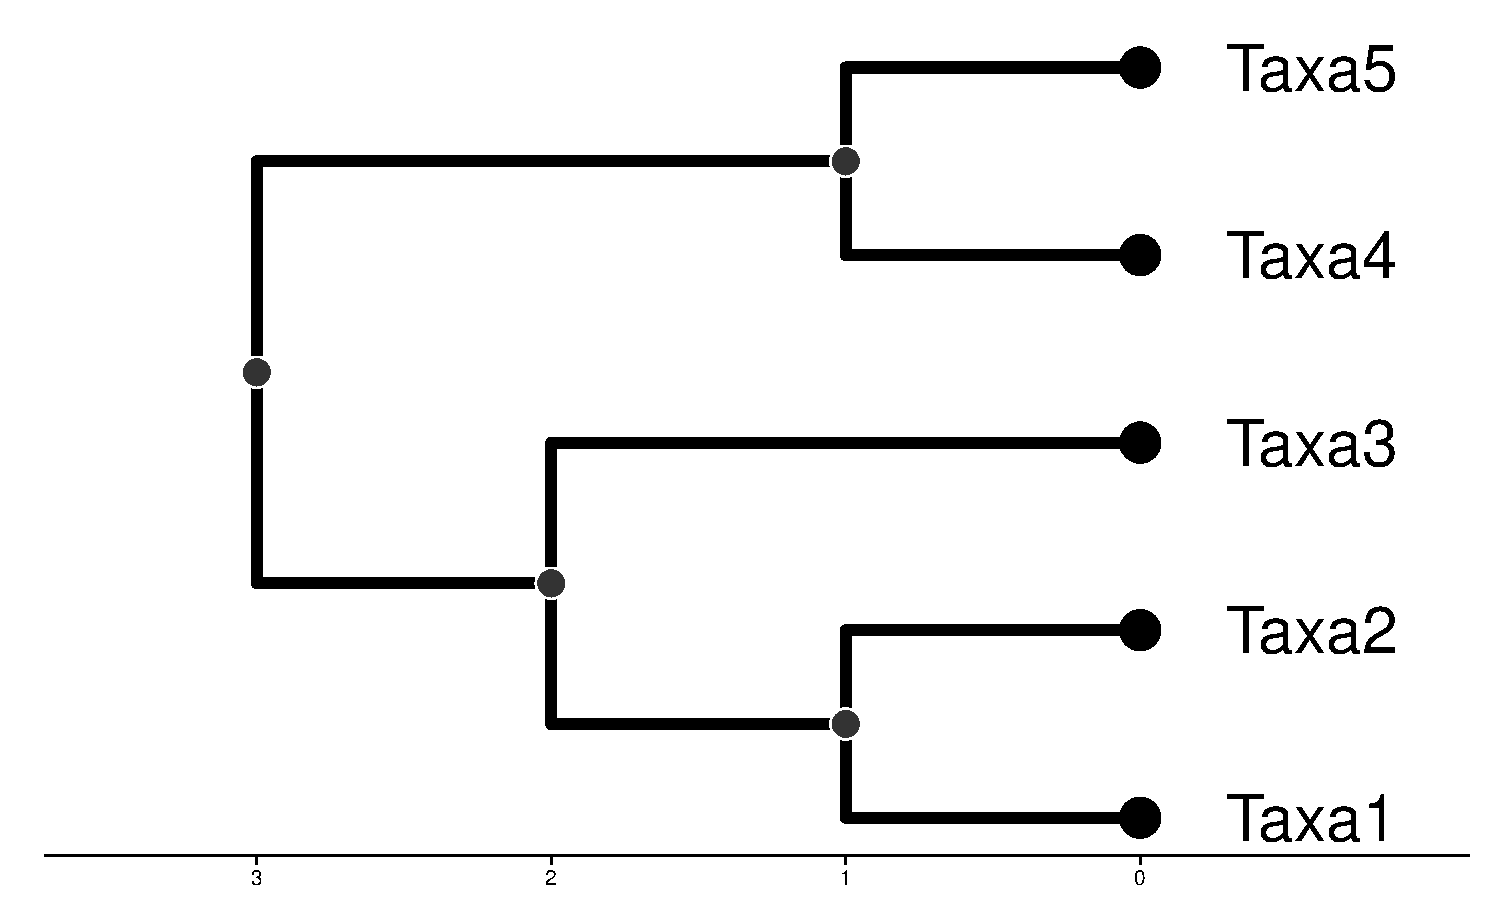
\includegraphics[scale=0.35]{treeconcept} 
\caption{
{ \footnotesize 
{\bf A phylogenetic tree showing evolutionary relationship.} Character sequences are observed at the tips of the tree (black dots); sequence characters at the internal nodes are treated as missing data (outlined dots). 
Branch lengths can be estimated in units of genetic distance, or as in this case, real time.
} % END: footnotesize
}
\label{fig:treeconcept}
\end{figure}

Within our framework we focus on trees which are rooted and time-measured, i.e. their branch lengths are scaled in actual time units.
A rooted binary tree with $n$ leaves has $2n-2$ branches and $n-1$ internal nodes.
The branching pattern of the tree is called the \emph{topology}. 

\subsection{Dated phylogenetic trees\label{sub:dated_trees}}

\myedit{svoneb}{
Time-stamped or `heterchronous' sequence data, which frequently arises from studies involving MEP populations for which sequences are sampled at different points in time and the evolutionary rates are high enough for significant changes to occur between the sampling times, can be used to calibrate the molecular clock and convert branch lengths into actual time units.
}
For simplicity let us assume a single site, where character sequence data was sampled on dates ranging from $1983$ to $2000$, as seen in Figure~\ref{fig:timing_sequences}.
We also assume that the rooted tree topology is known and we want to estimate the unknown times $T_{0},T_{6},T_{7},T_{8}$.

\begin{figure}[h!]
\centering
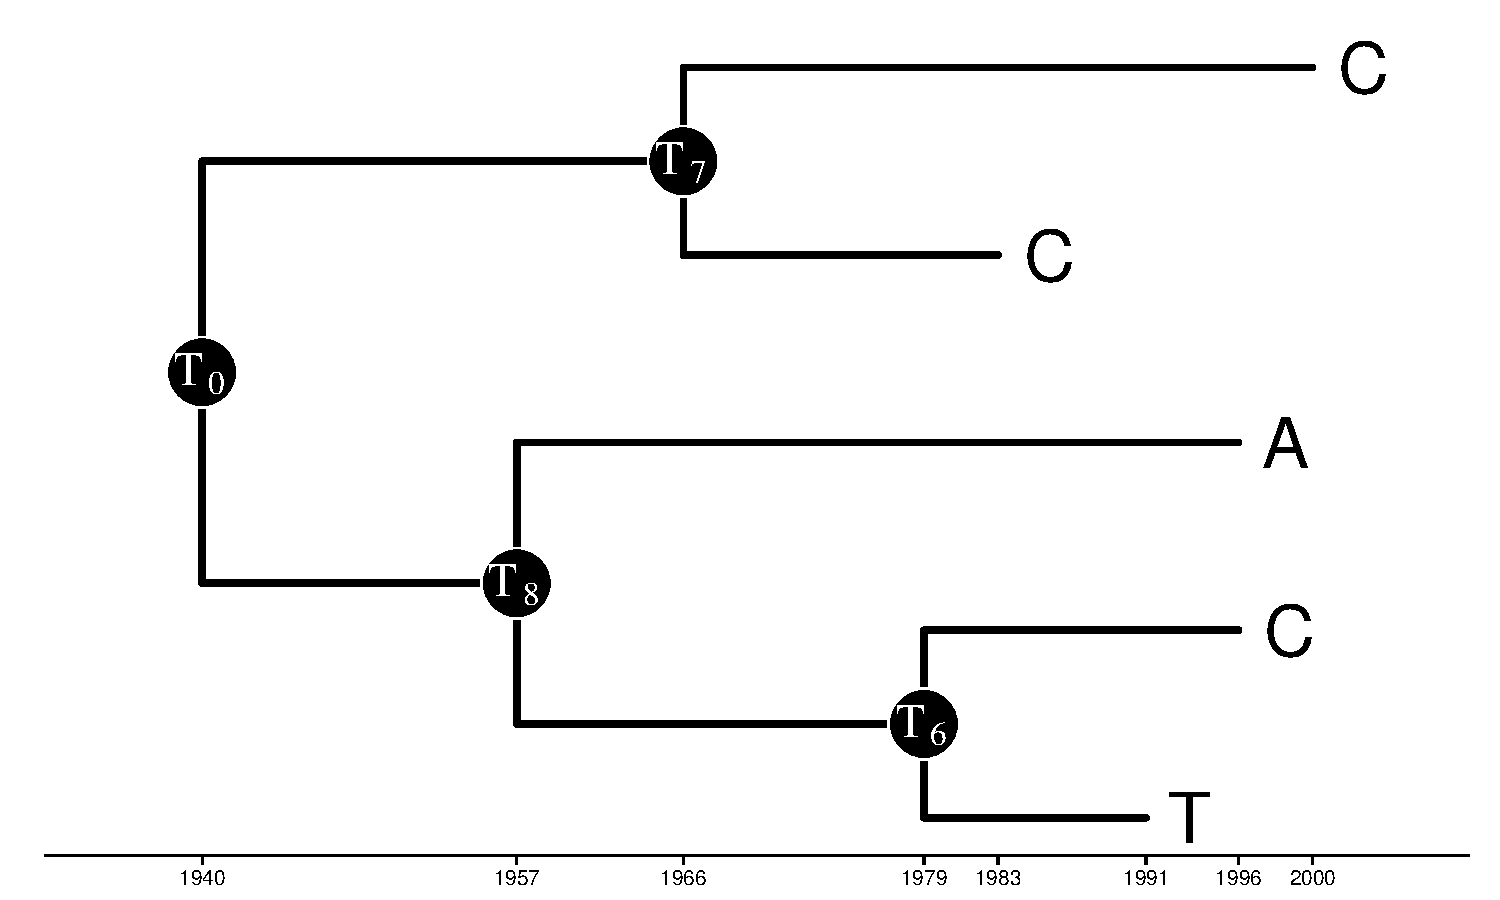
\includegraphics[scale=0.4]{timing_sequences} 
\caption{
{ \footnotesize 
{\bf Dated phylogenetic tree.} 
Discrete characters $CCACT$ observed at the external nodes (the tips of the tree) were sampled at different points in time.
The tree topology is assumed to be known without error, and also the root is known.
The unknown dates of the internal nodes are labelled $T_{0},T_{6},T_{7},T_{8}$.
}% END: footnotesize
}
\label{fig:timing_sequences}
\end{figure}

We start by estimating the rate of mutation $r$, which here is assumed to apply to the whole tree (a strict clock), from the differences in sampling times and the genetic distance, given by the model of sequence substitution.
This allows us to change the scale of the tree from units of substitutions to a time-scale measured in years.
The likelihood of the tree given estimated parameters $r,T_{0},T_{6},T_{7},T_{8}$ can be calculated using methods presented in Subsection~\ref{sub:likelihood}.


\subsection{Sequence evolution on a tree\label{sub:evolutionOnTree}}

In this section we proceed by describing the connection between the CTMC models of character substitution discussed above and phylogenetic histories.
We keep the focus on a single site of the alignment, and due to the assumption of independence the probability of observing an alignment is simply the product of probabilities for observing the individual sites.

To gain a better understanding of the process shaping the data observed at the tips of a phylogenetic tree let us consider the problem of simulating sequence evolution on a tree according to a model with rate matrix $\mathbf{Q}$.
We start with a first character $i$ sampled at the root of the tree $x_0$ from the stationary distribution $\mathbf{\Pi}$.
Let us assume that two direct descendent nodes are $x_j$ and $x_k$.
The character sampled at the root waits an exponentially distributed amount of time $t\geq0$ (see Figure~\ref{fig:poisson}) before moving to one of the descendent or child nodes.
Such traversal is said to be following the pre-order, i.e. parental nodes are visited before child nodes.   
The process then randomly decides by a coin flip to which of the two descendent nodes to move next (assuming that the visited node is not a tip).
Let us assume that the process moved to $x_j$.
The state $j$ for the node $x_j$ is sampled conditional on the value $i$ already sampled at the root using the branch length expressed in real time $t$ and the vector probabilities in the row $i$ of the finite-time probabilities matrix $\mathbf{P}(t)$, calculated using SVD of the rate matrix $\mathbf{Q}$ that characterizes the CTMC.   

\begin{algorithm}[h!]
\centering
\begin{algorithmic}[1]
% \footnotesize{
%
\State $node \gets getRoot\left(\right)$
%
\State $state \gets getState\left(node\right)$
%
\Repeat
%
\If{$\left(hasChildren\left(node\right)\right)$}
%
\ForAll{children}
%
\State $t \gets getDistanceToParent\left(child\right);$
%
\State $ \mathbf{P}\left(t\right) \gets e^{\mathbf{Q}t};$
%
\State $state \gets sample\left(\mathbf{P}\left[ state, \right]\right);$
%
\EndFor
%
\Else \Comment{this is a tip node}
%
\State $node \gets getParent\left(node\right);$
%
\EndIf
%
\Until{$\left(\text{simulated for all nodes}\right)$}
% }
\end{algorithmic}
\caption{
{ \footnotesize 
{\bf Pseudo code for simulating an evolutionary process along a phylogeny.} 
When a child node is visited, the state is sampled with conditional probabilities of changing to state $j$ given state $i$ at the parental node.
}% END: footnotesize
}
\label{alg:simulation}
\end{algorithm}

This illustrates the Markov property of a CTMC, as defined in Equation~(\ref{eq:markov}).
The sampling is then repeated on the node $x_j$, before recursively proceeding to the other trio of nodes.
The states sampled at the tips of the tree constitute the character sequence for one site of the alignment.
In this light the CTMC process can be viewed as a continuous-time random walk, unfolding on the topology $\mathbf{F}$, with its behaviour described by a rate-matrix $\mathbf{Q}$.
The complete algorithm is listed in Algorithm~\ref{alg:simulation}.

\section{Likelihood of sequence evolution}

\subsection{Calculation of the likelihood on a tree\label{sub:likelihood}}

The likelihood is defined as a conditional probability of observing the data given the parameters, as a function of those parameters.
%PL: mention perhaps Fisher, Edwards..?
Phylogenetic inference considers discrete molecular sequence data in the form of an aligned matrix $\mathbf{X}$ of size $n \times l$, where $x_{jh}$ is the $h$-th character in the $j$-th sequence.
A single column $\mathbf{x}_{h}$ of the data matrix constitutes a single site.
Again, the standard assumption of (site and lineage) independence posits that different sites evolve independently and that once two branches split at a node, the evolution on those branches is also independent.

In Subsection~\ref{sub:evolutionOnTree}, we described how evolution according to some process $\mathbf{Q}$ gives rise to the observed data $\mathbf{X}$.
Typically, we start with just the observed data and aim the inference efforts at modeling the process that generated the alignment.
We can therefore denote the likelihood simply as: 

\begin{equation}
L\left(\mathbf{\Theta}|\mathbf{X}\right)=P\left( \mathbf{X} | \mathbf{\Theta} \right), 
\label{eq:likelihood}
\end{equation}

\noindent
where $\mathbf{\Theta}$ represents the tree topology, the branch lengths, the parameters of the substitution model and other parameters of interest that we want to estimate.
This quantity expresses how likely it is to observe the data given a specific value of the parameter(s) of interest $\mathbf{\Theta}$.
\myedit{sveight}{
By finding the value of $\mathbf{\Theta}$ that maximizes (\ref{eq:likelihood}) we obtain an estimate of the most plausible 
%hypothesis for the data.
set of parameters given observed data.}

In this thesis we will not discuss maximum likelihood estimation itself, %PL: good, who wants to consider the data to be fixed anyway..
rather focus on closely related 
%PL: I would add: ".., but philosophically very different,"
% FB: difference: ML is an optimization procedure, Bayesian inference is a conditioning. It's a less aggresivee approach 
methods of Bayesian inference.
%GB: 'enters the framework as the data component' ? sounds weird, please rephrase
The likelihood concept is also required in Bayesian inference and enters the framework as the data component.
We will now discuss how to calculate the likelihood of observing a particular realization of character sequences at the tips of a tree, given a substitution model with fixed parameters.

%---LIKELIHOOD---%
\begin{figure}[h!]
\centering
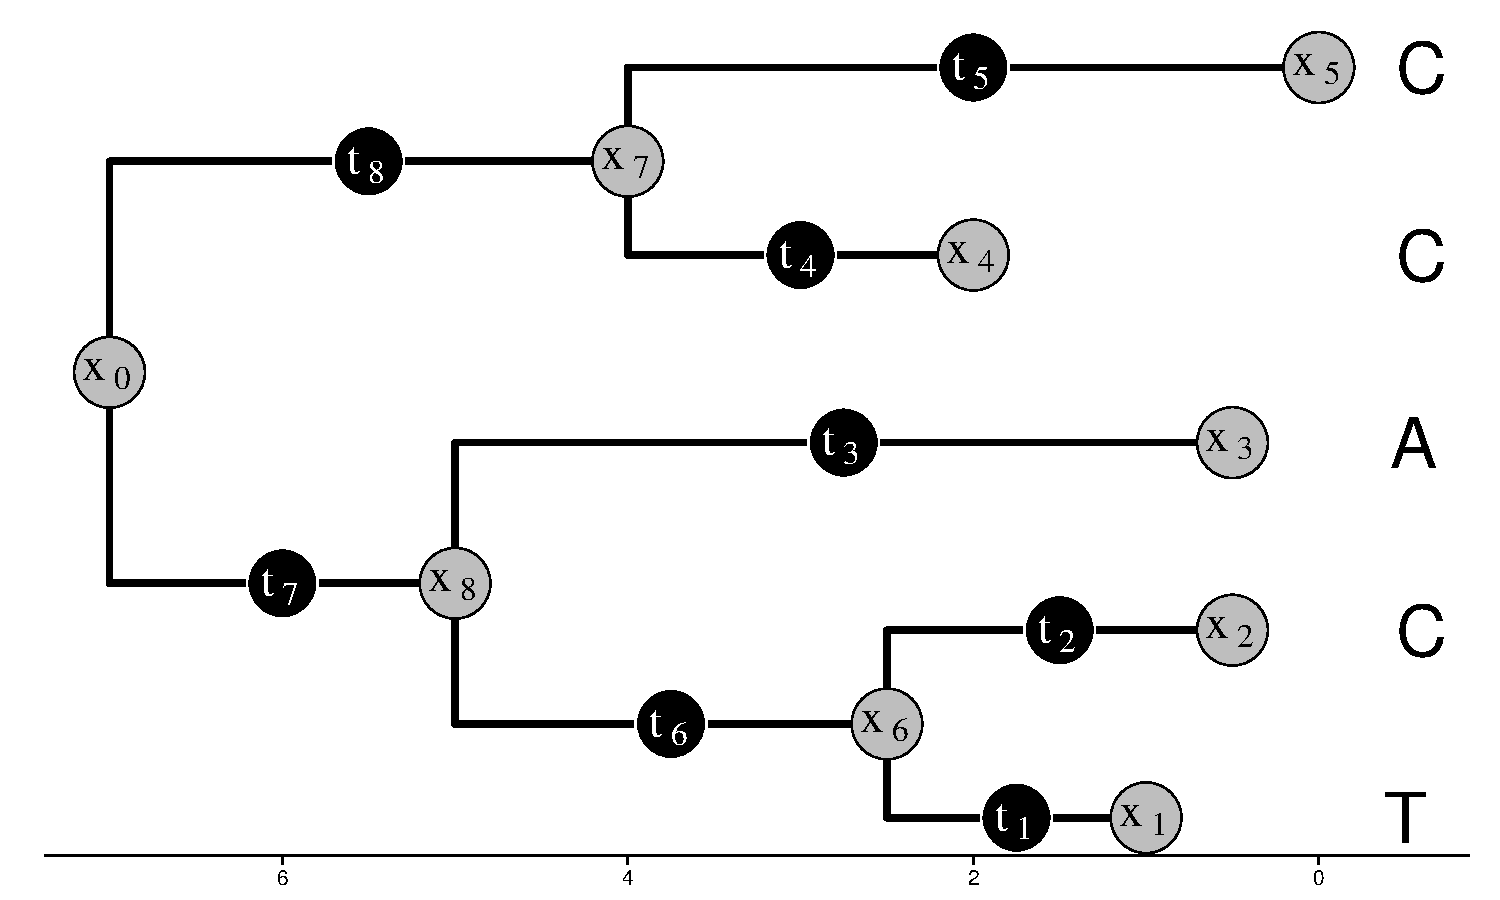
\includegraphics[scale=0.4]{likelihood} 
\caption{
{ \footnotesize 
{\bf  A hypothetical tree for five taxa.} Character data for a single site is observed at the tips of the tree.
} % END: footnotesize
}
\label{fig:LIKELIHOOD}
\end{figure}

To calculate the likelihood means in a sense to reverse-engineer the evolution as it happened.
Figure~\ref{fig:LIKELIHOOD} presents a single site with data $TCACC$ observed at the tips of the tree.
External nodes are numbered $x_{1}, \ldots x_{5}$, internal nodes $x_{6}, \ldots x_{8}$ and the root is placed at the node $x_{0}$.
The length of each branch leading to node $i$ is denoted as $t_{i}$. 
Using the methods presented in Subsection~\ref{sub:exponentiation}, we calculate the finite-time transition probabilities $p_{ij}(t_{i})$ between all pairs of characters in the alignment.
To calculate the probability at a single site, we need to sum over all possible combinations that could give rise to the observed character data at that site, in this case:

\begin{align}
\underset{x_{0}\in \mathcal{E}}{\sum}\;\underset{x_{6}\in \mathcal{E}}{\sum}\;\underset{x_{7}\in \mathcal{E}}{\sum}\;\underset{x_{8}\in \mathcal{E}}{\sum}[\pi_{x_{0}}\cdot p_{x_{0}x_{8}}(t_{7})\cdot p_{x_{0}x_{7}}(t_{8})\cdot p_{x_{8}x_{6}}(t_{6})\cdot p_{x_{8}A}(t_{3}) \nonumber \\
\cdot p_{x_{7}C}(t_{4})\cdot p_{x_{7}C}(t_{5})\cdot p_{x_{6}T}(t_{1})\cdot p_{x_{6}C}(t_{2})].
\label{eq:likelihoodNaive}
\end{align}

We can break down the terms in Equation~(\ref{eq:likelihoodNaive}) 
to the probability of observing the data $TCACC$ for the tips and $x_{0},x_{6},x_{7},x_{8}$ for the ancestral nodes (inside the brackets) and the sum over all possible path combinations over the state space $\mathcal{E}$ (outside the brackets).
Term $\pi_{0}$ is simply the probability that the root has character $x_{0}$ and is based on the assumption that the process generating the data has reached its equilibrium.

Summing over all possible paths leading to the observed data is computationally expensive, as there are  $K^{n-1}$ possible combinations, where $n-1$ is the number of internal nodes of a rooted binary tree.
Fortunately, we can rely on the assumption of independence of the process in the two sub-trees below every node.
Based on this, \citet{Felsenstein1981} provides an efficient algorithm for computing the likelihood of observing the data on a topology $\mathbf{F}$ given the substitution model that quantifies transition probabilities.
This routine, known as \emph{tree pruning}, conveniently expresses the partial likelihood $L_{i}(x_{i})$ of observing data at the descendants of node $i$ given state $x_{i}$ at node $i$ in terms of partial likelihoods at nodes $j$ and $k$.
For all internal nodes of $\mathbf{F}$ we have:

\begin{equation}
L_{i}(x_{i})=\left[\underset{x_{j}\in \mathcal{E}}{\sum}\mathbf{P}_{x_{i}x_{j}}(t_{j})L_{j}(x_{j})\right]\times\left[\underset{x_{k}\in \mathcal{E}}{\sum}\mathbf{P}_{x_{i}x_{k}}(t_{k})L_{k}(x_{k})\right]
\label{eq:felsenstein1}
\end{equation}

\noindent
For tip nodes we have:

\begin{equation}
L_{i}(x_{i})=\begin{cases}
1 & \text{if }\hat{x}(i)=x_{i}\\
0 & \text{otherwise}
\end{cases},
\label{eq:felsenstein2}
\end{equation}

\noindent
where $\hat{x}(i)$ denotes the character state observed at node $i$.
After recursively applying (\ref{eq:felsenstein1}) to all the nodes of $\mathbf{F}$ in post-order fashion, the likelihood of the data at the site is given by:
% we can integrate out the unobserved states calculating successive contributions to the partial likelihood.

\begin{equation}
L(\mathbf{x}_{h})=\underset{x_{0}\in\mathcal{E}}{\sum}\pi_{x_{0}}\cdot L_{0}(x_{0})
\label{eq:felsenstein3}
\end{equation}

\noindent
In most applications for computational reasons is is easier to work with the natural logarithm of the likelihood in Equation~\ref{eq:felsenstein3}.
Thanks to the assumption of site-independence, the log-likelihood of the whole alignment $X$ can be computed by summing the logarithms of the likelihoods at the particular sites:

\begin{equation}
l(X)=\underset{j=1}{\overset{l}{\sum}}log\left(L(\mathbf{x}_{jh})\right)
\label{eq:loglikelihood}
\end{equation}

\subsection{The computational burden of likelihood computations\label{sub:mlburden}}

We have already mentioned that for large data sets the run-time of statistical phylogenetic analysis is a major hurdle that hampers the development and application of novel, more biologically relevant models and inference in the field.
These limits are being actively stretched, for example by porting the computationally expensive calculations to high-performance parallel computing devices such as Graphics-Processing Units (GPUs, \cite{Nickolls2008}).
In Subsection~\ref{sub:exponentiation}, we already discussed how the computation of finite-time transition probabilities can be reduced to simple matrix algebra operations, which can be handled by high-performance libraries and APIs for statistical phylogenetics such as the BEAGLE library \citep{Ayres2012, Suchard2009}. 

%GB: do we need this computational complexity section? Not sure if we want to go into that much detail ...
Before we proceed with discussing the burden imposed by certain steps when calculating the likelihood of a sequence evolution on a tree, we need a formal definition of the computational complexity of a sequential routine.
The efficiency of an algorithm can depend on various factors, like network usage, disk usage, operational memory usage or CPU real-time usage.
All of these factors should be taken into consideration when designing and implementing a computational routine. 
However, for most of the calculations the CPU time will be the rate-limiting factor.
Typically both mathematicians and computer scientists use the Big-O notation as a relative representation of algorithm complexity, like the execution time required.
Here we formally define the Big-O notation as:

\begin{definition}
Let us assume two functions $f:\mathbb{R}_{>0}\rightarrow\mathbb{R}_{>0}$ and $T:\mathbb{R}_{>0}\rightarrow\mathbb{R}_{>0}$. 
For $n \in \mathbb{R}_{>0}$ we write:

\begin{equation}
T(n) \in \mathcal{O}\left(f(n)\right)
\label{eq:bigOh}
\end{equation}

\noindent
if and only if there exists a constant $M>0$ and some $n_0 \in \mathbb{R}_{>0}$ such that:

\begin{equation}
\forall n\geq n_{0}\;T(n)\leq M \cdot f(n)
\end{equation}
\end{definition}


% \noindent
In other words $T(n)$, which can be interpreted as the ``worst-case'' time complexity of an algorithm,
% Since an algorithm's performance time may vary with different inputs of the same size
is $\mathcal{O}\left(f(n)\right)$ if and only if for all sufficiently large input values $T(n)$ is bounded from above by some constant multiple of $f(n)$.
This makes the Big-O notation useful when analyzing algorithms for run-time efficiency and makes it possible to, for example, compare routines without the added overhead of negligible terms, such as the architecture at which the code was run, the choice of language or compiler.
We will now briefly discuss some of the most common serial computational orders and their examples. 

\begin{algorithm}[h!]
\centering
\begin{algorithmic}[1]
% \footnotesize{
\State $a \gets \text{\textbf{new int}}$;
%
\If{ $\left(a == 1 \right)$ }
%
\State \textbf{return} $true$;
%
\Else 
%
\State \textbf{return} $false$;
%
\EndIf
% }
\end{algorithmic}
\caption{
{ \footnotesize 
{\bf Single test operation.} 
} % END: footnotesize
}
\label{alg:o1}
\end{algorithm}

The simplest, most basic example is an operation that takes the same amount of time every time it is called, thus requiring constant time, i.e. it's computational complexity is that of $\mathcal{O}\left(1\right)$ and does not depend on the input size.
An example of such routine is listed in the Algorithm~\ref{alg:o1} that evaluates a specific value of a constant.

\begin{algorithm}[h!]
\centering
\begin{algorithmic}[1]
% \footnotesize{
\State $a \gets \text{\textbf{new int}}\left[n\right]$;
%
\For{int $\left(i=0; \; i<a.size(); \; i++\right)$}
%
\If{ $\left(a\left[i\right] == 1 \right)$ }
%
\State \textbf{return} $true$;
%
\Else 
%
\State \textbf{return} $false$;
%
\EndIf
%
\EndFor
% }
\end{algorithmic}
\caption{
{ \footnotesize 
{\bf Search for a value.} 
}% END: footnotesize
}
\label{alg:on}
\end{algorithm}

An algorithm proceeding at $\mathcal{O}\left(N\right)$ has a run-time that grows linearly with the size of input data.
An example of such a routine is presented as Algorithm~\ref{alg:on}, which searches an array looking for a specific value.
We should note that the Big-O notation always describes the performance in worst-case scenario, i.e. a full loop has to be executed before a matching element is found, while for the actual real-world problem this does not have to be the case and the loop can return earlier.

\begin{algorithm}[h!]
\centering
\begin{algorithmic}[1]
% \footnotesize{
\State $a \gets \text{\textbf{new int}}\left[n\right]$;
%
\For{int $\left(i=0; \; i<a.size(); \; i++\right)$}
%
\For{int $\left(j=0; \; j<a.size(); \; j++\right)$}
%
\If{ $\left(i == j \right)$ }
%
\State \textbf{do nothing};
%
\Else 
%
\If{ $a\left[ i \right] == a\left[ j \right]$ }
%
\State \textbf{return} $true$;
%
\EndIf
%
\EndIf \Comment{END: i == j check}
%
\EndFor \Comment{END: j loop}
%
\EndFor \Comment{END: i loop}
% }
\end{algorithmic}
\caption{
{ \footnotesize 
{\bf Search for the first duplicated value.} 
}% END: footnotesize
}
\label{alg:on2}
\end{algorithm}

An algorithm can also require a quadratic run-time, $\mathcal{O}\left(N^2\right)$, i.e. its performance is directly proportional to the square of the size of the input data.
Among examples of such an algorithm is the routine that searches for a duplicated value in an array, and requires two nested loops as presented in Algorithm~\ref{alg:on2}.
Similarly, nesting more loops will result in routines which proceed at polynomial times $\mathcal{O}\left(N^3\right)$, $\mathcal{O}\left(N^4\right)$, $\mathcal{O}\left(N^5\right)$, etc.
An algorithm proceeding at $\mathcal{O}\left(c^N\right)$, where $c>1$ is some constant, will have a run-time that grows c-times with every additional data element, i.e. exponentially. 

Having described these basic concepts, we can now come back to the original problem of calculating the likelihood of sequence evolution on a fixed tree.
From Subsections \ref{sub:exponentiation} and \ref{sub:likelihood} we already know the steps involved:

% I skipped site rate variability, but perhaps it should be mentioned? 
\begin{enumerate}
\item { Singular value decomposition of the rate matrix $\mathbf{Q}$. }
\item { Taking the exponential of $\mathbf{Q}t$ for each branch length $t$. }
\item { Applying Equation~(\ref{eq:felsenstein1}) for every site in the alignment and every possible state in the state space $\mathcal{E}$. }
\item { Taking the logarithm of the likelihood for every site and summing over all sites in the alignment. }
\end{enumerate}

Step (i) proceeds at ${\cal{O}}(K^3)$; however, for typical, time-homogeneous applications this is not the rate-limiting step, as repeated evaluations of $\exp(\mathbf{Q}t)$ in (ii) are based on the same decomposition of the matrix \citep{Suchard2009}. 
Step (ii) typically boils down to repeated matrix-vector-matrix multiplications and its serial computational order is ${\cal{O}}(K^3 \times n)$. 
Step (iii) takes ${\cal{O}}(K^2 \times n \times l)$ time and is the most computationally expensive part of the routine. 
Step (iv) proceeds at ${\cal{O}}(l)$, linearly with the number of sites.
Fortunately, these operations are very regular and lend themselves to exploit computational parallelism, such as utilized in the BEAGLE library \citep{Suchard2009,Ayres2012}.

% TODO: maybe sub-section on GPUs here

\section{Bayesian inference\label{sec:bayesian_inference}}

\subsection{Bayesian evolutionary analysis}

The Bayesian approach to statistical inference combines prior information with the data to generate the posterior distributions of the parameters of interest.
All other post-hoc inference is based on those generated posterior distributions.
Bayesian methodology has recently gained immense popularity, due to the advances in numerical algorithms and the progressively cheaper access to powerful computational hardware.
The development of statistical programs for simulation from Bayesian hierarchical models like OpenBUGS \citep{Lunn2009} and JAGS \citep{Plummer2003} has also helped to bolster the popularity and accessibility of the Bayesian framework.

In the field of phylogenetics, Bayesian inference has been applied to some of the most complex problems and is now widely adopted, with the term \emph{Bayesian evolutionary analysis} used to describe molecular evolutionary analyses set in the Bayesian framework.
At the forefront of these advancements lies the active development and wide adoption of popular Bayesian evolutionary analysis software packages like MrBayes \citep{Ronquist2012} and BEAST \citep{Drummond2012}.

\subsection{Bayes theorem\label{sub:bayesTheorem}}

% Following the notation defined in Subsection \ref{sub:likelihood} we will denote the tree topology, the branch lengths and the parameters of the substitution model that we aim at inferring by $\mathbf{\Theta}$.
Following the notation defined in Subsection~\ref{sub:likelihood}, let us denote a single-dimensional parameter of interest that we aim to learn about as $\theta$.
The central concept of Bayesian inference is that this parameter has a distribution of its own.
Before the molecular data $\mathbf{X}$ is observed we assume that $\theta$ has a prior distribution $P(\theta)$.
The prior reflects the prior beliefs about the possible values of the parameter.

\myedit{svnine}{
The prior choice is perhaps one of the most controversial points of the Bayesian inference.
The prior distributions may come from the preceding analysis of other sets of data, or they may form some set of biologically plausible values.
However in some cases there may be no suitable objective distribution at hand, in which case one often resorts to the so-called \emph{vague} or \emph{diffuse} priors, which have large variances.
Some popular uninformative priors on continuous, unbounded variables may be improper, \textit{i.e.} their distribution is infinitesimal on an infinite range in order to integrate to $1$.
Among examples of such priors is the uniform distribution on an infinite interval.
Although many of of these prior choices sill lead to a proper posterior distribution, yet some controversies about their choice may still arise.
}

% TODO: discuss hyperpriors?
The prior information is then combined with the likelihood of the data $P\left( \mathbf{X} | \theta \right)$ to form the posterior, via Bayes' theorem (Equation~(\ref{eq:bayesian1})).
The posterior distribution of $\theta$ follows:

\begin{align}
P\left(\theta|\mathbf{X}\right) &= \frac{P(\theta)\cdot P\left(\mathbf{X}|\theta\right)}{P\left(\mathbf{X}\right)}=\frac{P(\theta)\cdot P\left(\mathbf{X}|\theta\right)}{\int P(\theta)\cdot P\left(\mathbf{X}|\theta\right)d\theta}  \nonumber \\
& \approx  P(\theta)\cdot P\left(\mathbf{X}|\theta\right),
\label{eq:bayesian1}
\end{align}

\noindent
where the marginal probability of the data $P\left(\mathbf{X}\right)$ is a normalizing constant that makes the posterior $P\left(\theta|\mathbf{X}\right)$ integrate to one.
The last approximation in Equation~(\ref{eq:bayesian1}) means that the posterior is proportional to the prior times the likelihood.

% nuisance parameters? GB: I second that
Bayesian inference provides a natural way of dealing with nuisance parameters.
Suppose that $\mathbf{\Theta}=\left(\theta,\mathbf{F}\right)$ is now a two dimensional vector of parameters, with $\theta$ being the parameter of interest, while 
$\mathbf{F}$ (e.g. a tree topology) is the nuisance parameter.
The joint posterior distribution of $\mathbf{\Theta}$ is now:

\begin{eqnarray}
P\left(\mathbf{\Theta}|\mathbf{X}\right) &=& P\left(\theta,\mathbf{F}|\mathbf{X}\right)=\frac{P\left(\theta,\mathbf{F}\right)\cdot P\left(\mathbf{X}|\theta,\mathbf{F}\right)}{P\left(\mathbf{X}\right)}  \nonumber \\
&=& \frac{P\left(\theta,\mathbf{F}\right)\cdot P\left(\mathbf{X}|\theta,\mathbf{F}\right)}{\int\int P(\theta,\mathbf{F})\cdot P\left(\mathbf{X}|\theta,\mathbf{F}\right)d\theta d\mathbf{F}}
\label{eq:bayesian2}
\end{eqnarray}

\noindent
and the marginal posterior density of $\theta$ can be obtained from Equation~\ref{eq:bayesian2} as:

\begin{equation}
P\left(\theta|\mathbf{X}\right) =\int P\left(\theta,\mathbf{F}|\mathbf{X}\right)d\mathbf{F}
\label{eq:bayesian3}
\end{equation}

\subsection{Example: Comparing two sequences with the beta-binomial model\label{sub:ex_beta_binom}}

As a simple illustration of the concept of Bayesian analysis, let us consider a toy example where two sequences are compared and $x=10$ differences are found out of $N=100$ sites compared.
Suppose that the parameter $\theta$ we want to infer is the proportion of sites which differ between the two sequences.
Assuming that the sites are independent we can use a binomial model and put a beta prior with parameters $\alpha=2$, $\beta=100$ on the unknown proportion $\theta$, suggesting that \textit{a priori} we prefer small values of the $\theta$ parameter.

%---POSTERIOR PRIOR LIKELIHOOD---%
\begin{figure}[h!]
\centering
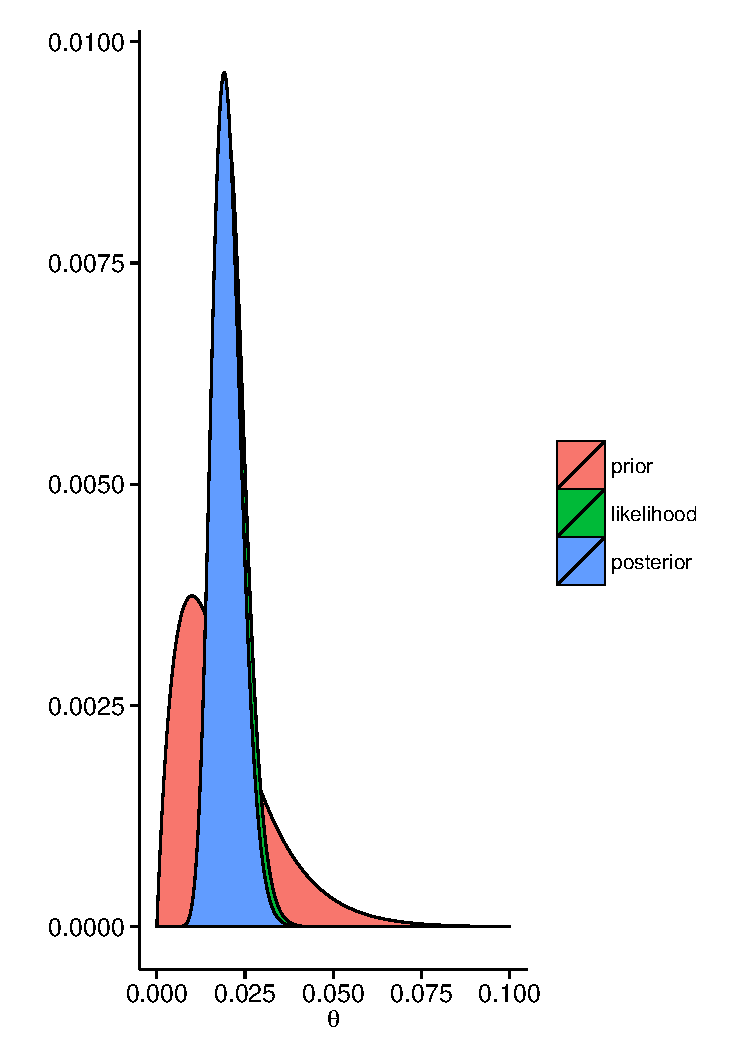
\includegraphics[scale=0.45]{bayes} 
\caption{
{ \footnotesize 
{\bf Beta(2,100) prior and posterior densities plotted with a scaled likelihood resulting from a binomial model.} 
}% END: footnotesize
}
\label{fig:bayes1}
\end{figure}

Figure~\ref{fig:bayes1} shows the resulting posterior distribution along with prior and scaled likelihood.
The likelihood of the binomial model used in this example is simply:

\begin{align}
L\left(\theta|x\right)=\left(\begin{array}{c}
N\\
x
\end{array}\right)\theta^{x}(1-\theta)^{N-x}
\label{eq:binomial_like}
\end{align}

Equation~\ref{eq:binomial_like} is plotted in Figure~\ref{fig:bayes1} over a range of values of $\theta$, resulting in the black filled distribution.
The Beta distribution we chose for the prior has a following distribution function:

\begin{align}
p(\theta)=\frac{1}{B\left(\alpha,\beta\right)}\theta^{\alpha-1}(1-\alpha)^{\beta-1}
\label{eq:beta_dist}
\end{align}

Equation~\ref{eq:beta_dist} corresponds to the white filled curve in in Figure~\ref{fig:bayes1}.
Following the Bayes rule from Equation~\ref{eq:bayesian1} we can combine the likelihood and prior to form the posterior, which then becomes:

\begin{eqnarray}
p\left(\theta|x\right)=& \frac{\left(\begin{array}{c}
N\\
x
\end{array}\right)\theta^{x}(1-\theta)^{N-x}\times\frac{1}{B\left(\alpha,\beta\right)}\theta^{\alpha-1}\left(1-\theta\right)^{\beta-1}}{\int\left(\begin{array}{c}
N\\
x
\end{array}\right)\theta^{x}(1-\theta)^{N-x}\times\frac{1}{B\left(\alpha,\beta\right)}\theta^{\alpha-1}\left(1-\theta\right)^{\beta-1}d\theta} \nonumber \\
=& \frac{1}{B\left(\alpha+x,\beta+N-x\right)}\theta^{\alpha+x-1}(1-\theta)^{\beta+N-x-1}
\label{eq:beta_binom_post}
\end{eqnarray}
 
Equation~\ref{eq:beta_binom_post} appears as a grey filled area in Figure~\ref{fig:bayes1}.
This illustrates that the data `pulls' the posterior away from the prior, and the strength by which is does so depends on its variance, resulting in a posterior centered around 0.06 in this case.
In this example, the posterior distribution can be obtained analytically because the beta distribution is a so-called \emph{conjugate prior} for the binomial model, resulting in the posterior that is also beta-distributed.












\subsection{Markov Chain Monte Carlo\label{sub:mcmc} }

Except for the most trivial problems, involving conjugate priors as in our previous example, the calculation of the integral in Equation~(\ref{eq:bayesian1}) poses a considerable challenge in Bayesian inference.
This integral leads to the marginal probability of the data $P\left(\mathbf{X}\right)$. 
For even the simplest phylogenetic problems, one has to integrate over all possible tree topologies, all of the branch lengths in those trees and all of the substitution parameters in the applied model.
Such highly-dimensional integrals are impossible to calculate analytically.
This is where the Markov Chain Monte Carlo (MCMC) algorithm shows its strength and provides a powerful method of sampling from the posterior distributions without having to evaluate the marginal probability. %PL: it is a supa-dupa algorithm: http://oldweb.cecm.sfu.ca/~jborwein/algorithms.html

The Metropolis-Hasting algorithm, as proposed by \citet{Metropolis1953}, is an MCMC algorithm for sampling from multi-dimensional distributions.
It proceeds by constructing a Markov chain with its states being the values of the parameter of interest $\theta$ and whose equilibrium distribution is the posterior $P\left(\theta|\mathbf{X}\right)$ as defined in Equation~\ref{eq:bayesian1}.
After choosing an arbitrary starting state for the chain, new candidate states $\theta^{*}$ are generated from the proposal density, also called the kernel, $q(\theta^{*} | \theta[t]), \; t=1,\ldots,M$, where $M$ is the chain length and $\theta[t]$ is the current value of the chain.

A common kernel choice to propose new state for continuous parameter is to sample from a uniform distribution centered around the current state of the chain, the so-called sliding window kernel: 

$$\theta^{*}\sim U\left[\theta[t]-\omega,\theta[t]+\omega\right], \; t=1,\ldots,M,$$

\noindent
where $\omega$ is the arbitrary window size.
The chain then moves to the proposed value with probability defined by the acceptance ratio (see Equation~(\ref{eq:metropolis1})), or if the proposal is rejected the chain remains at the current state.
The routine iterates between accept/reject steps for a specified number of times.
Both acceptance and rejection are counted as iterations of the algorithm; in fact the rejections ensure that the probabilistic properties of the target distribution are well represented in the generated sample.  
Algorithm~\ref{alg:metropolisHastings} presents the details of the Metropolis-Hastings algorithm.

\begin{algorithm}[h!]
\centering
\begin{algorithmic}[1]
% \footnotesize{
%
\State Pick a starting value of the chain $\theta \left[ t \right]$ for $t=0$.
%
\For{int $\left(t=1; \; t<M-1; \; t++\right)$}
%
\State Generate a candidate state from the proposal distribution (kernel):
$$\theta^{*} \sim q(\theta[t])$$
%
\State Calculate the acceptance ratio:
$$r=\frac{prior\left(\theta^{*}\right)}{prior\left(\theta\left[t\right]\right)}\cdot\frac{Likelihood\left(\mathbf{X}|\theta^{*}\right)}{Likelihood\left(\mathbf{X}|\theta\left[t\right]\right)}\cdot\frac{q\left(\theta\left[t\right]|\theta^{*}\right)}{q\left(\theta^{*}|\theta\left[t\right]\right)}.$$
%
\State Sample $u\sim U[0,1]$.
%
\If{$\left( u < r \right)$}
%
\State Set $\theta[t+1]=\theta^*.$
%
\Else 
%
\State Set $\theta[t+1]=\theta[t].$
%
\EndIf
%
\EndFor
% }
\end{algorithmic}
\caption{
{ \footnotesize 
{\bf The Metropolis-Hastings algorithm} 
}% END: footnotesize
}
\label{alg:metropolisHastings}
\end{algorithm}

Several important features of the algorithm can be noted.
The most important part of the algorithm is the proposal density. 
Given the current state it proposes the next state independent of the past states.
We can recall that this is the Markov property, in fact the output of the algorithm generates a Markov chain, hence the name MCMC.
The Metropolis-Hastings algorithm allows for the use of an asymmetrical proposal densities such that $q\left(\theta\left[t\right]|\theta^{*}\right)\neq q\left(\theta^{*}|\theta\left[t\right]\right)$.
The acceptance probability is simply the ratio of the target posterior evaluated at the proposal and at the current state of the chain, times the ratio of the proposal: 
% prior ratio times the likelihood ratio times the proposal ratio

% \myedit{DPseven}{
\begin{equation}
\frac{P\left(\theta^{*}|\mathbf{X}\right)\cdot q\left(\theta\left[t\right]|\theta^{*}\right)}{P\left(\theta\left[t\right]|\mathbf{X}\right)\cdot q\left(\theta^{*}|\theta\left[t\right]\right)}=\frac{P(\theta^{*})\cdot P\left(\mathbf{X}|\theta^{*}\right)\cdot q\left(\theta\left[t\right]|\theta^{*}\right)}{P(\theta\left[t\right])\cdot P\left(\mathbf{X}|\theta\left[t\right]\right)\cdot q\left(\theta^{*}|\theta\left[t\right]\right)}.
\label{eq:metropolis1}
\end{equation}
% }

Note that the integral in Equation~(\ref{eq:bayesian1}) which is notoriously hard to compute cancels out in (\ref{eq:metropolis1}).
Hence, to estimate the posterior $P\left(\theta|\mathbf{X}\right)$ one only needs to run the algorithm for a sufficiently long time to let the chain reach its equilibrium, which is precisely the target posterior.
%PL: maybe mention that this can be formally proven using the ergodic theorem... and no, you don't have to prove it in the appendix ;-)

\subsection{Example: Estimating genetic distances}

Let us revisit the toy example in which we compare two sequences and find $x=10$ differences among $n=100$ sites.
This time however we will use MCMC to estimate the genetic distance between the two sequences using the Jukes and Cantor model of nucleotide substitution (see Subsection~\ref{sub:jc69}).
Genetic distance is defined as the expected number of substitutions per nucleotide site, which we will denote as $\theta=rt$ in line with previous sections, where $r$ is the substitution rate (see Subsection~\ref{sub:poisson}) and $t$ is the evolutionary time separating the two sequences.
The time and rate are generally confounded as we already mentioned, and hence they will be estimated as a single parameter of interest $\theta$.
The probability that the descendant nucleotide in a sequence is different from the ancestral nucleotide can be obtained by summing over all possible paths, between two pairs of nucleotides, i.e. $p_{ij}(t)=\underset{k\neq i}{\sum}p_{ik}(t)$.

From Equation~(\ref{eq:jc69Finite}) in Subsection~\ref{sub:jc69}, we know that under the JC69 model those probabilities are all equal, therefore the probability that a single site is different between two sequences separated by distance $\theta=rt$ is given by:

\begin{equation}
p=3p_{1}\left(t\right)=\frac{3}{4}\left(1-e^{\left(-4/3\right)\theta}\right).
\label{eq:distance1}
\end{equation}

\noindent
From this we can formalize the likelihood function using the binomial model given that we observe $x$ differences out of $n$ sites :

\begin{equation}
P\left(\mathbf{X}|\theta\right)=L\left(\mathbf{X}|\theta\right)=\left(\begin{array}{c}
n\\
k
\end{array}\right)p^{x}(1-p)^{n-x},
\label{eq:likelihood1}
\end{equation}

\noindent
where $p$ is as defined by Equation~(\ref{eq:distance1}).
We use an exponential prior on $\theta$ with mean $1/\lambda$:

\begin{equation}
P\left(\theta,\lambda\right)=\frac{1}{\lambda}e^{-(1/\lambda)\theta},
\label{eq:expPrior}
\end{equation}

\noindent
and set $\lambda=10$.
For the proposal we choose a uniformly distributed jumping kernel with a window size of $w=0.1$.

%---METROPOLIS PATH---%
\begin{figure}[h!]
\centering
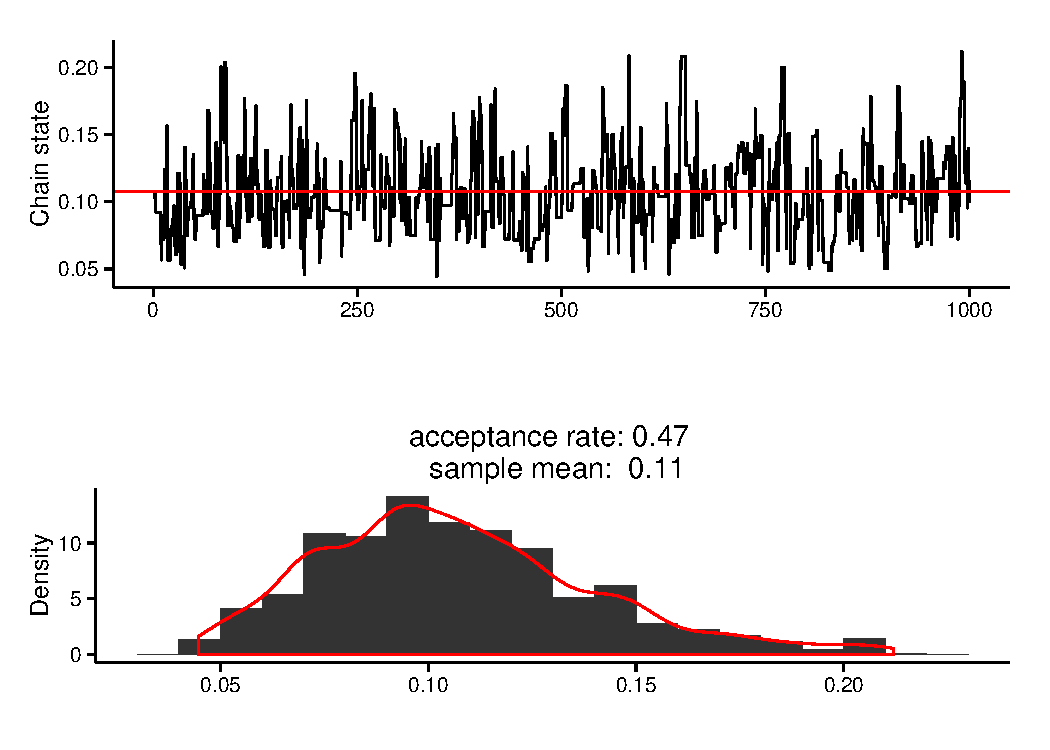
\includegraphics[scale=0.5]{metropolis} 
\caption{
{ \footnotesize 
{\bf MCMC output for estimating the genetic distance under the JC69 model.}
Trace plot in the upper panel results from a direct implementation of Algorithm~\ref{alg:metropolisHastings}.
The likelihood is calculated under the binomial model, with probabilities coming from the JC69 nucleotide substitution model. 
We put an exponential prior on the parameter $\theta$.
With the grey line we indicate the MLE estimator of $\theta$. 
In the lower panel we plot the posterior density estimated using MCMC.
}% END: footnotesize
}
\label{fig:metropolis}
\end{figure}

Figure~\ref{fig:metropolis} shows $1000$ iterations of the chain generated by Algorithm~\ref{alg:metropolisHastings} in the upper plot and applied to the genetic distance problem.
The grey line indicates the maximum likelihood estimate (MLE) $\hat{\theta}$ of parameter $\theta$ which is calculated by setting $\frac{d\ell\left(\mathbf{X}|\theta\right)}{d\theta}=0$, where $l\left(\mathbf{X}|\theta\right)$ is the logarithm of likelihood defined by Equation~(\ref{eq:likelihood1}):

\begin{equation}
\hat{\theta}=\frac{3}{4}log\left(1-\frac{4}{3}\cdot\frac{x}{n}\right)
\label{eq:mle}
\end{equation}

In the lower plot of Figure~\ref{fig:metropolis} we can see an estimate of the posterior density, along with the sample mean.
The posterior sample mean is identical to the MLE up to the second decimal place, although we have not run the chain for long.
The acceptance rate is high, suggesting that almost as many steps are accepted as are rejected.
%GB: acceptance rates don't necessarily have to be this high, not sure if you want to discuss this though.

For reference we now repeat the same procedure, yet this time we set the window size to $w=1.0$.
The resulting time-series plot is presented in Figure~\ref{fig:window_size}.

%---WINDOW SIZE---%
\begin{figure}[h!]
\centering
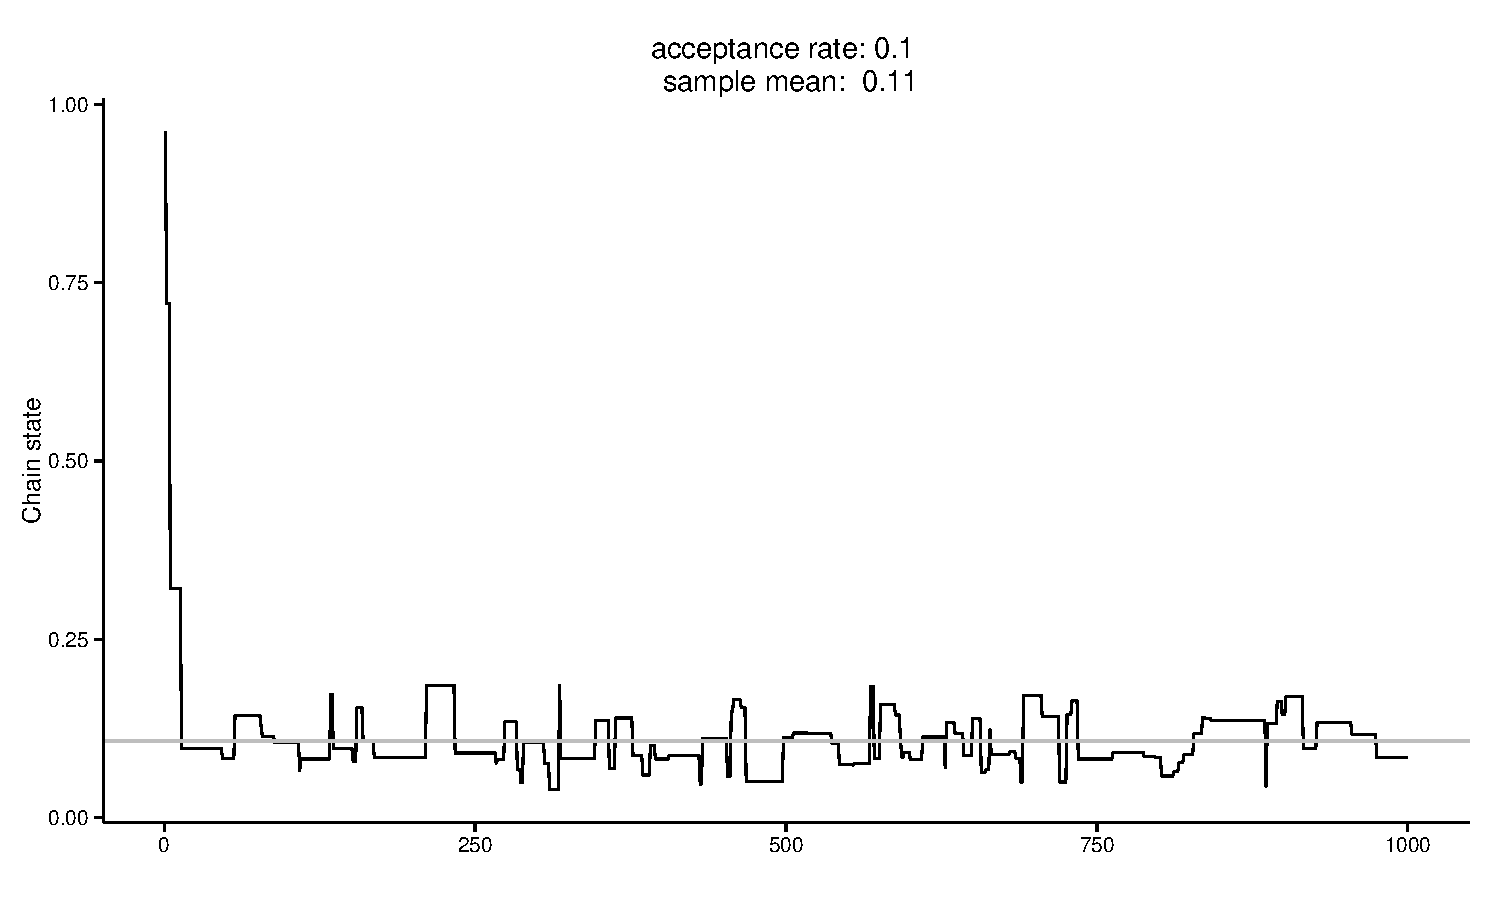
\includegraphics[scale=0.5]{window_size} 
\caption{
{ \footnotesize 
{\bf MCMC output for the same problem as presented in Figure~\ref{fig:metropolis}, with proposal having the window size of $1.0$.}
}% END: footnotesize
}
\label{fig:window_size}
\end{figure}

It is clear from the plot that the proposal is sub-optimal in this case; the large window does not allow for the posterior to be efficiently explored, leading for too many moves to be rejected, which is also apparent when looking at the acceptance rate.
However, this does not mean that the algorithm fails, as it will still reach its stationary distribution \citep{Tierney1994}, although it needs much more samples to do so than the proposal in Figure~\ref{fig:metropolis}. 
For a given sample size a more efficient proposal will produce more samples from the posterior distribution.
The efficiency of the sampler, as measured by the acceptance rate, can thus be viewed as a measure of accuracy of the inferences.

Even for the most basic problems the convergence needs to be formally assessed.
If the iterations of the MCMC algorithm, such as M-H, have not proceeded for long enough, the collected sample may not be representative of the true posterior (target) distribution.
%GB: the term 'sequences' is not a good choice here I think
One recommended approach for assessing convergence of the chain is to compare different simulated calculations starting from different initial values in terms of their within and between chain variance, an approach known as the Gelman and Rubin diagnostics \citep{Cowles1996}. 
If the within chain variation is much less than the between chain variation, the different calculations have clearly not converged.
The weighted average of those variances is then taken as an estimate of the variance of the stationary distribution and is guaranteed to be an unbiased estimator if the starting values come from the stationary distribution.

Trace plots such as the ones in Figures~\ref{fig:metropolis} and~\ref{fig:window_size} are a useful visual aid for assessing the mixing of a single chain.
Density estimates, like the histogram in the bottom panel of Figure~\ref{fig:metropolis} can also help in spotting the most apparent mixing problems that the particular chain might have.
Convergence assessment procedures can only reliably diagnose situations in which the particular chain has failed to converge in the given simulation time, yet they do not guarantee the converse; i.e. that the chain which seems like a convergent one has in fact explored the whole target distribution.

There have been many propositions for improving the convergence of the chain to the equilibrium distribution, see for example \cite{Liu1994, Gelfand1995, Vines1996}.
Even if the MCMC simulations have reached convergence, early collected iterations are still influenced by the starting value.
To reduce the impact of those, the general practice is to discard the first $10\%$ of the collected samples, often referred to as the \textit{burn-in}.

Another problem that frequently arises is inherited from the iterative nature of the algorithm, i.e. the within sequence correlations.
Although not a problem for convergence, as after reaching the target distribution the sampled values are guaranteed to be \textit{iid}, it poses an efficiency problem.
If the collected sequences are used directly to estimate the posterior distribution of the unknown parameter the estimates are generally less efficient, because of that auto correlation.
The Effective Sample Size (ESS) is a frequently used measure of the information that the collected sample size contains.
One of the techniques for reducing auto correlation is called \textit{thinning}, which skips every $k$-th iteration from the sampled sequence. 

\subsection{Bayesian phylogeography\label{sub:phylogeo}}

Phylogeography is a research direction aimed at connecting evolutionary processes, which happen over time, with the processes of spatial dispersal into a joint spatio-temporal dynamic that can be used to track pathogen spread.
%GB: I don't like the use of 'reciprocal' here ...
% FB: could also use complementary
Historically, phylogeographic inference in molecular epidemiology ignored the correlated nature of these two processes. 
The evolutionary relationships represented by the tree were inferred were first estimated from the sequence data, and then the ancestral locations generated by the process of the spatial diffusion were reconstructed from the spatial data, conditioning on the inferred tree topology.
\citet{Lemey2009} first considered the Bayesian reconstruction that allows for joint inference of both a time-measured evolutionary history and the parameters of the spatial and temporal process that shapes the spread and evolution of 
% e.g. 
rapidly evolving viruses.
This approach does not require fixing the tree topology, the branch lengths nor the Markov model parameters, and allows for integration over all possible values, requiring only for a specification of a prior distributions for the parameters that we aim to infer.

\myedit{svonec}{
Central to the Bayesian phylogeographic framework is the hypothesis that sequence evolution is occurring simultaneously with the process of geographical dispersal. 
The observed data, residing at the $N$ tips of phylogeny $\mathbf{F}$, is recorded as both character sequence data $\mathbf{X}=(X_{1},...,X_{N})$ and discretized geographic locations (countries, districts, cities) $\mathbf{Y}=(Y_{1},...,Y_{N})$, as depicted in the upper facet of Figure~\ref{fig:discrete_phylo_illust}.
We assume independent stochastic processes are responsible for generating these data, with ancestral states of $\mathbf{X}$ generated as before by a CTMC characterized by rate matrix $\mathbf{Q}$ and the unobserved ancestral locations $(Y_{N+1},...,Y_{2N-2})$ generated by a separate CTMC characterized by rate matrix $\mathbf{\Phi}$ (see Figure~\ref{fig:discrete_phylo_illust}, lower facet).
The entries of this matrix are the transition rates $\phi_{ij}$ between locations $i$ and $j$.
Unlike before, the rate matrix does not necessarily have to be symmetrical, i.e. there exist some $i,j$ such that $\phi_{ij}\neq\phi_{ji}$.
Additionally, a priori one would expect many of the infinitesimal rates to be zero. 
}

%---DISCRETE PHYLOGEOGRAOHY ILLUSTRATION---%
\begin{figure}[h!]
\centering
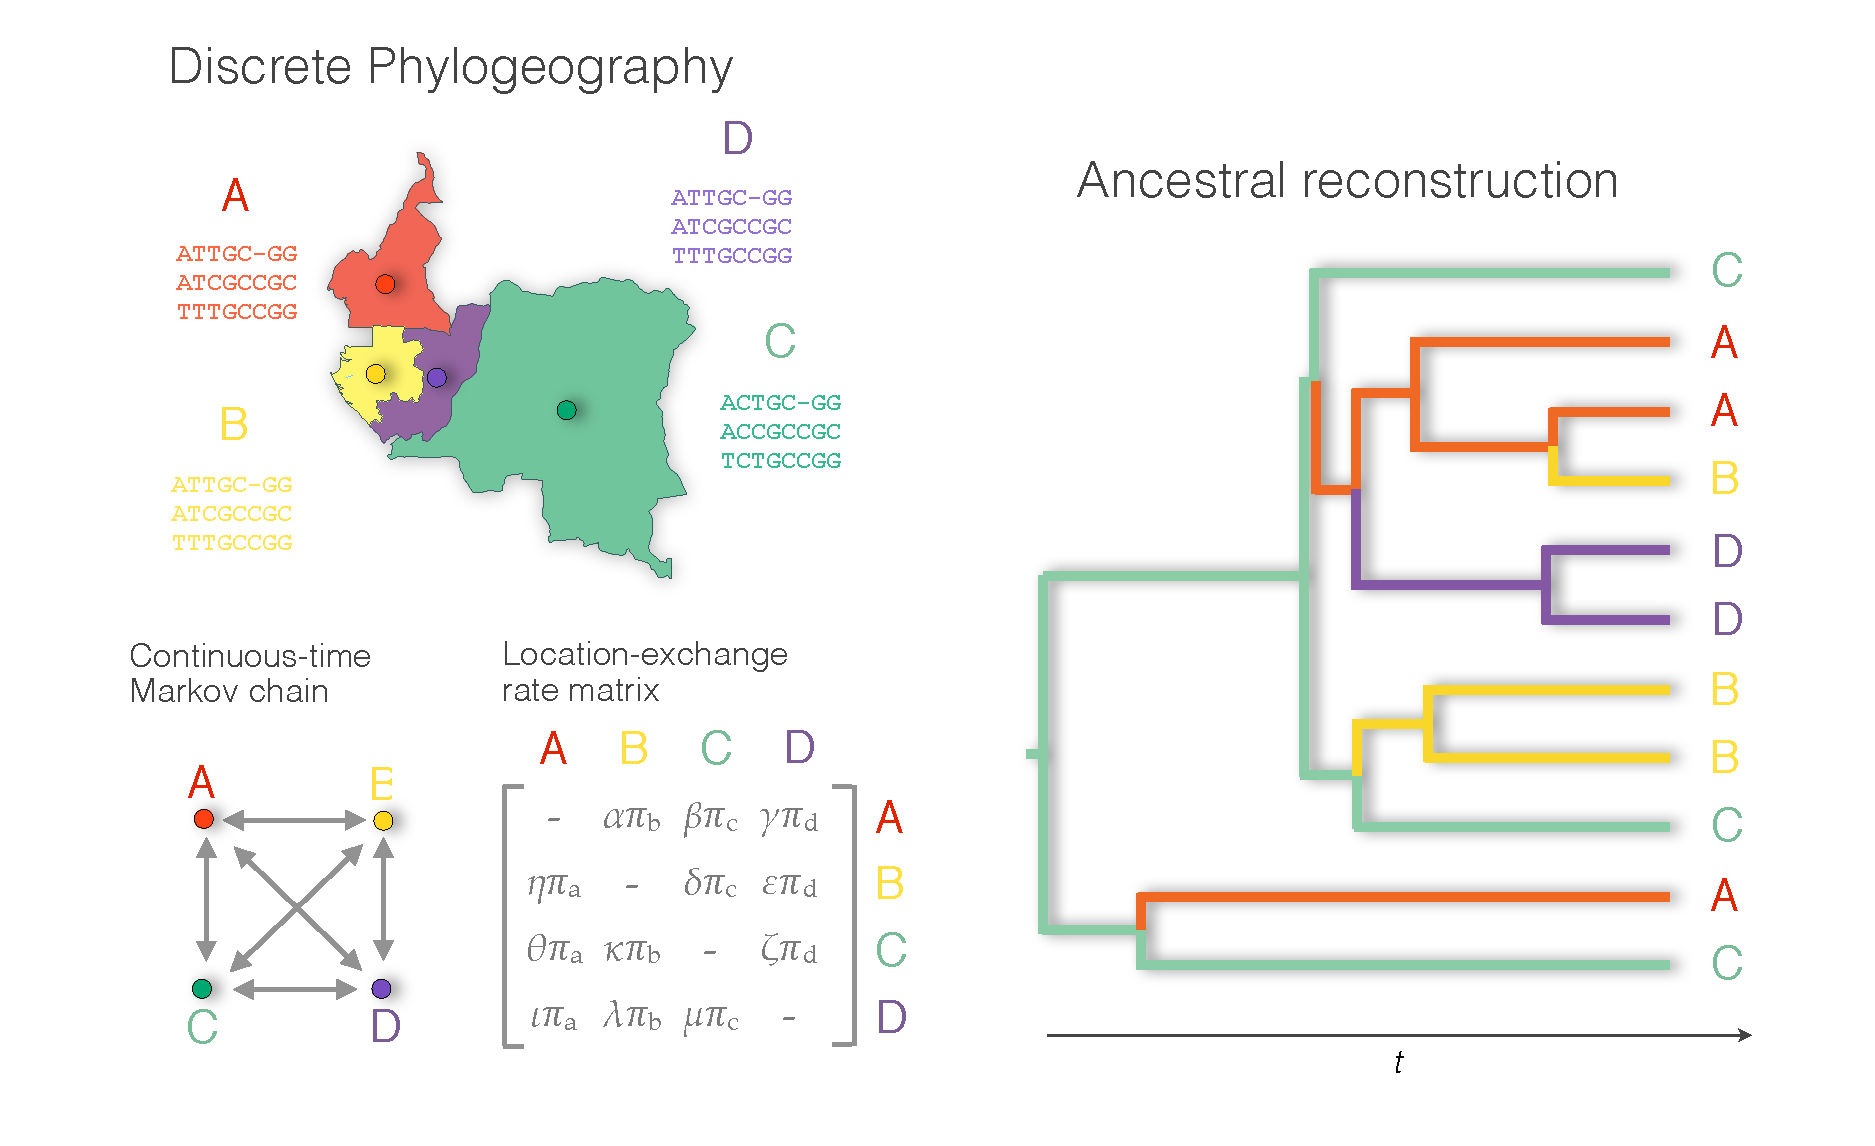
\includegraphics[scale=0.4]{discretePhylogeography} 
\caption{
{ \footnotesize 
{\bf Discrete phylogeographical model for $K=4$ location states.} 
The data consist of both the character sequences and locations at which they were recorded.
The model allows for non-symmetric rates of location exchange in the evolutionary history.
}% END: footnotesize
}
\label{fig:discrete_phylo_illust}
\end{figure}


Unlike the molecular data, which is typically dense, the location data is sparse, with only one observation per taxon and many transitions are likely to remain observed.
For this reason, a Bayesian stochastic search variable selection (BSSVS, see also Subsection~\ref{sub:clocks}) procedure has been proposed in order to allow exchange rates in $\mathbf{\Phi}$ that do not contribute to the phylogeographic diffusion to shrink to zero with a certain probability.

The Bayesian framework described in Subsections~\ref{sub:bayesTheorem} and \ref{sub:mcmc} offers the unique ability to integrate different sources of information about the viruses with their genetic data, without conditioning on either one of them.
We use this ability to infer the tree topology, the ancestral spatial locations and the character substitution process giving rise to the aligned molecular sequence data. 
Since assume independent stochastic processes are responsible for generating these data, we can write down the joint posterior distribution as: 

\begin{align}
P\left(\mathbf{F}, \mathbf{Q}, \mathbf{\Phi}|\mathbf{X},\mathbf{Y}\right) &\propto 
\underbrace{P(\mathbf{X}|\mathbf{Q}, \mathbf{F})}_{\begin{array}{c}
\substack{\text{Sequence} \\ \text{likelihood}}
\end{array}}\cdot\underbrace{P(\mathbf{Y}|\mathbf{\Phi}, \mathbf{F})}_{\begin{array}{c}
\substack{\text{Trait} \\ \text{likelihood}}
\end{array}}\cdot
\underbrace{P(\mathbf{F})}_{\begin{array}{c}
\substack{\text{Topology} \\ \text{prior}}
\end{array}} \nonumber \\
& \cdot \underbrace{P(\mathbf{Q})}_{\begin{array}{c}
\substack{\text{Sequence substitution} \\ \text{prior}}
\end{array}}\cdot\underbrace{P(\mathbf{\Phi})}_{\begin{array}{c}
\substack{\text{Location exchange} \\ \text{prior}}
\end{array}}
\label{eq:posteriorPhylogeography}
\end{align}

The likelihood component for both molecular data $\mathbf{X}$ and location data $\mathbf{Y}$ is calculated using recursive tree pruning, as described in Subsection~\ref{sub:likelihood}.
We approximate the joint posterior as written down in Equation~(\ref{eq:posteriorPhylogeography}) using MCMC methods we discussed in Subsection~\ref{sub:mcmc}, which leads to the reconstruction of the most plausible histories with ancestral location states, as depicted in the left facet of the Figure~\ref{fig:discrete_phylo_illust}.

In order to study phylogeographic processes based on longitude and latitude coordinates of sampled strains, Brownian motion has been proposed as the random walk model in continuous space with conceptually very similar inference procedures \citep{Lemey2010}.


\subsection{Bayesian model selection\label{sub:model_selection}}
% https://radfordneal.wordpress.com/2008/08/17/the-harmonic-mean-of-the-likelihood-worst-monte-carlo-method-ever/

A standard approach to compare models in a Bayesian phylogenetic framework is through the evaluation of Bayes factors (BFs).   
The BF is a ratio of two marginal likelihoods, which given the observed data $\mathbf{X}$ quantify the plausibility of two models, denoted $M_{1}$ and $M_{2}$ and are parametrised in terms of parameters $\theta_{1}$ and $\theta_{2}$ respectively:

% 
\begin{equation}  
\frac{\int P\left(\mathbf{X}|\theta_{1},M_{1}\right)\times P\left(\theta_{1} \mid M_{1}  \right)d_{\theta_{1}}}{\int P\left(\mathbf{X}|\theta_{1},M_{2}\right)\times P\left(\theta_{2} \mid M_{2} \right)d_{\theta_{2}}},
\label{eq:bayes_factor}
\end{equation}  
% 

\noindent
where $P\left(\mathbf{X}|\theta_{i},M_{i}\right)$ is the likelihood function and $P\left(\theta_{i} \mid M_{i} \right)$ is the prior, for $i=1, 2$.
The parameters $\theta_{i},\; i=1, 2$ can be possibly multidimensional, making the integral in Equation~\ref{eq:bayes_factor} non-trivial to estimate.
For a number of years the posterior Harmonic Mean Estimator (HME, \cite{Newton1994}) has been extensively used in Bayesian phylogenetic inference, mainly for the simplicity in its calculation. 
To evaluate the HME one only needs the samples from the posterior distribution which are readily available as output form any MCMC program.

Among others, \cite{Meng1996}, \cite{Lartillot2006} and \cite{Xie2011} warn that despite this computational convenience the HME is a biased estimator of the (log) marginal likelihood, severely overestimating the true value and with potentially infinite variance.
%GB: not typically the correct references for this type of work, so I removed them
This has lead to a substantial amount of work invested in the development of more accurate methods for estimating (log) marginal likelihoods.
To this end, \cite{Lartillot2006} introduced path sampling (PS) into the field of phylogenetics, providing several examples for which the HME was drastically outperformed by PS when estimating the marginal likelihood.
The authors showed that even for simple Gaussian examples, for which the true value of the marginal likelihood can be analytically calculated, the HME was unable to estimate the true underlying value whereas PS proved very reliable for all cases examined. 
Further, for evolutionary models with high dimensions, the HME severely overestimated the (log) marginal likelihood compared to PS, leading to a plausible explanation for many dubious findings concerning model selection over the years.

Recently, \cite{Xie2011} developed stepping-stone sampling (SS) as a computationally more interesting alternative to path sampling (PS).
The authors show that by essentially performing the same calculations as for PS, but using the collected samples in a different way, they are able to compose a more efficient (log) marginal likelihood estimator.
Both PS and SS rely on drawing MCMC samples from a series of distributions, each of which is a power posterior differing only in its power, along the path going from the prior to the unnormalized posterior defined by the model $M$:  

\begin{equation}  
q_{\beta}\left(\theta\right)=P\left(\mathbf{X}\mid\theta,M\right)^{\beta} \times P\left(\theta\mid M\right).
\label{eq:ss_ps}
\end{equation}  

\cite{Baele2012} have performed a comparative study on the performance of HME, the stabilized/smoothed HME (sHME), the AICM (a posterior simulation-based analogue of Akaike?s information criterion through Markov chain Monte Carlo, PS and SS in a phylogenetic framework.
The authors showed that PS and SS consistently outperformed the harmonic mean estimators as well as the AICM when comparing demographic models as well as relaxed clock models.
Although offering tremendous improvements in bias and variance over the HME both PS and SS require considerable computational effort as the (log) marginal likelihood can no longer be estimated from the likelihood trace that is being output from the standard MCMC analysis. 
Further, great care must also be taken to specify proper priors for all parameters in Equation~\ref{eq:ss_ps}, so as to avoid numerical instabilities when the integration approaches the prior \cite{Baele2013b}.  











